%\documentclass[table]{article}
%\usepackage{beamerarticle}
\documentclass[10pt,xcolor=table,ignorenonframetext,aspectratio=169]{beamer}
%\documentclass[10pt,xcolor=table,ignorenonframetext]{beamer}
\mode<presentation>
{
  \usetheme{default}
  \useoutertheme{split}
% \usefonttheme{serif}
}

\usenavigationsymbolstemplate{}
\usepackage{amssymb}
\usepackage{amsmath}
\usepackage{setspace}
\usepackage{graphicx}
\usepackage{multirow}
\usepackage[english]{babel}
\usepackage[latin1]{inputenc}
\usepackage{bm}
\usepackage{graphicx}
\usepackage{multirow}
\usepackage{tikz}
\usepackage[english]{babel}
\usepackage[latin1]{inputenc}
%\usepackage{ulem}
\usepackage{pifont}
\usepackage{changepage}
%\usepackage{colortbl}
%\usepackage[table]{xcolor}
%\usepackage{xcolor}

\setbeamersize{text margin left=1cm,text margin right=5cm}

\setbeamertemplate{itemize item}[circle]
\setbeamertemplate{frametitle}[default][center]

\newlength{\wideitemsep}
\setlength{\wideitemsep}{\itemsep}
\addtolength{\wideitemsep}{4pt}
\let\olditem\item
\renewcommand{\item}{\setlength{\itemsep}{\wideitemsep}\olditem}

\newcommand{\HRule}{\rule{0.5\textwidth}{0.05mm}}

\usetikzlibrary{arrows,positioning,shapes}
\usetikzlibrary{decorations.pathreplacing}

\definecolor{blueish}{RGB}{97,156,255}
\definecolor{greenish}{RGB}{0,186,56}
\definecolor{reddish}{RGB}{248,118,109}

\definecolor{oiverm}{RGB}{213,94,0}
\definecolor{oiblue}{RGB}{0,114,178}
\definecolor{oigreen}{RGB}{0,158,115}
\definecolor{oipurple}{RGB}{204,121,167}
\definecolor{oiorange}{RGB}{230,159,0}
\definecolor{oisky}{RGB}{86,180,233}
\definecolor{oiyellow}{RGB}{240,228,66}
\definecolor{williams}{RGB}{81,38,152}

\definecolor{hue1}{RGB}{255,255,204}
\definecolor{hue2}{RGB}{161,218,180}
\definecolor{hue3}{RGB}{65,182,196}
\definecolor{hue4}{RGB}{44,127,184}
\definecolor{hue5}{RGB}{37,52,148}

\definecolor{dvg1}{RGB}{213,62,79}
\definecolor{dvg2}{RGB}{244,109,67}
\definecolor{dvg3}{RGB}{253,174,97}
\definecolor{dvg4}{RGB}{254,224,139}
\definecolor{dvg5}{RGB}{230,245,152}
\definecolor{dvg6}{RGB}{171,221,164}
\definecolor{dvg7}{RGB}{102,194,165}
\definecolor{dvg8}{RGB}{50,136,189}

\setbeamercolor{structure}{fg=williams,bg=williams!12}

\title{Diff-in-Diff in a Regression Framework, Slide \insertframenumber}
\subtitle{}

\author{Economics 379 (Professor Jakiela)}
\date{}



\begin{document}
	
	
	
%%%%%%%%%%%%%%%%%%%%%%%%%%%%%%%%%%%%%%%%%%%%%%%%%%%%%%%%%%%%%%%%%%%%%%%%%%
	% COURSE Title slide
%%%%%%%%%%%%%%%%%%%%%%%%%%%%%%%%%%%%%%%%%%%%%%%%%%%%%%%%%%%%%%%%%%%%%%%%%%
	
\begin{frame}<beamer:0>[plain]
	
	\begin{center}
		\begin{tikzpicture}
		
		\node [opacity=1] (bg)  {\includegraphics[keepaspectratio,height=0.9\paperheight]{photos/Kenya-cistern-Flore-de-Preneuf-2011-LARGE.jpg}};
		
		\node [anchor=east,align=right] at (6,-2.25) {\Large{\textcolor{white}{Williams College ECON 379:}}};		
		\node [anchor=east,align=right] at (6,-3) {\Large{\textcolor{white}{Program Evaluation for International Development}}};

		\node [anchor=east] at (6,-3.8) {\textcolor{yellow}{\tiny{photo:  Flore de Preneuf / World Bank}}};
		
		\end{tikzpicture}
	\end{center}
\end{frame}


%%%%%%%%%%%%%%%%%%%%%%%%%%%%%%%%%%%%%%%%%%%%%%%%%%%%%%%%%%%%%%%%%%%%%%%%%%
% LECTURE Title slide
%%%%%%%%%%%%%%%%%%%%%%%%%%%%%%%%%%%%%%%%%%%%%%%%%%%%%%%%%%%%%%%%%%%%%%%%%%

\begin{frame}[plain]

\only<beamer>{\begin{adjustwidth}{0cm}{-4cm}}

\begin{center}
	\begin{tikzpicture}
	
	\node [opacity=0.25] (bg)  {\includegraphics[keepaspectratio,height=0.9\paperheight]{photos/Senegal-WAAPP-seeds-Daniella-Van-Leggelo-Padilla-LARGE.jpg}};
	
	\node at (0,2.5) {\large{\textcolor{williams}{Williams College ECON 379:}}};		
	\node at (0,1.5) {\large{\textcolor{williams}{Program Evaluation for International Development}}};
	
	\node at (0,-0.5) {\large{\textcolor{williams}{\textbf{Module 5: Diff-in-Diff in a Regression Framework}}}};
	
	\node at (0,-2) {\large{\textcolor{williams}{Professor:  Pamela Jakiela}}};
	
	\node [anchor=east] at (6,-3.8) {\textcolor{yellow}{\tiny{photo:  Daniella Van Leggelo-Padilla / World Bank}}};
	
	\end{tikzpicture}
\end{center}
\only<beamer>{\end{adjustwidth}}
\end{frame}



%%%%%%%%%%%%%%%%%%%%%%%%%%%%%%%%%%%%%%%%%%%%%%%%%%%%%%%%%%%%%%%%%%%%%%%%%%%

%\begin{frame}<handout:0>[bg,plain]
\begin{frame}[plain]

\only<beamer>{\begin{adjustwidth}{0cm}{-4cm}}

\begin{center}
	
\Large{$2\times2$ Diff-in-Diff Specifications}
	
\end{center}

\only<beamer>{\end{adjustwidth}}
\end{frame}


%%%%%%%%%%%%%%%%%%%%%%%%%%%%%%%%%%%%%%%%%%%%%%%%%%%%%%%%%%%%%%%%%%%%%%%

\begin{frame}{Difference-in-Differences Estimation}


\begin{center}
	\begin{tikzpicture}
	
	% blank canvas
	\only<handout>{\fill[fill=white,draw=white,ultra thin]
		(0,0) -- (11,0) -- (11,6) -- (0,6) -- cycle;}
	\only<beamer>{\fill[fill=white,draw=white,ultra thin]
		(0,0) -- (14,0) -- (14,6) -- (0,6) -- cycle;}
	\only<beamer>{\draw[draw=oiblue!60,fill=oiblue!10,opacity=0.5] (11,1) rectangle (14,5);}
	%\draw[step=1.0,gray!20,thin] (0,0) grid (11,6);
	
	\pgfmathsetmacro\xshift{5cm};
	\pgfmathsetmacro\yshift{3.5cm};
	
	% highlight cells
%	\pgfmathsetmacro\mycolor{"oigreen!32"};
%	\filldraw[\mycolor,xshift=\xshift,yshift=\yshift,opacity=0.4] (-2,-2) -- (-2,1.75) -- (0,1.75) -- (0,-2) -- cycle;
%	\pgfmathsetmacro\mycolor{"oiyellow!64"};
%	\filldraw[\mycolor,xshift=\xshift,yshift=\yshift,opacity=0.4] (2,-2) -- (2,1.75) -- (0,1.75) -- (0,-2) -- cycle;
%	\pgfmathsetmacro\mycolor{"red!32"};
%	\filldraw[\mycolor,xshift=\xshift,yshift=\yshift,opacity=0.4] (-4.5,-1) -- (-4.5,-2) -- (4,-2) -- (4,-1) -- cycle;
	
	% 2X2 grid with labels
	\pgfmathsetmacro\mycolor{"black"};
	\node[\mycolor,anchor=east,align=right,xshift=\xshift,yshift=\yshift] at (-2,0.5) {\small{pre}};
	\node[\mycolor,anchor=east,align=right,xshift=\xshift,yshift=\yshift] at (-2,-0.5) {\small{post}};
	\node[\mycolor,anchor=east,align=right,xshift=\xshift,yshift=\yshift] at (-2,-1.5) {\small{difference}};
	\node[\mycolor,anchor=south,xshift=\xshift,yshift=\yshift] at (-1,1.0) {\small{\textcolor{white}{p}treatment\textcolor{white}{p}}};
	\node[\mycolor,anchor=south,xshift=\xshift,yshift=\yshift] at (1,1.0) {\small{\textcolor{white}{p}comparison\textcolor{white}{p}}};
	\node[\mycolor,anchor=south,xshift=\xshift,yshift=\yshift] at (3,1.0) {\small{\textcolor{white}{p}difference\textcolor{white}{p}}};
	\draw[\mycolor,thick,xshift=\xshift,yshift=\yshift] (-3.75,-2) -- (4,-2) -- (4,1) -- (-3.75,1) -- cycle;
	\draw[\mycolor,thick,xshift=\xshift,yshift=\yshift] (-2,-2) -- (4,-2) -- (4,1.75) -- (-2,1.75) -- cycle;
	\draw[\mycolor,thick,xshift=\xshift,yshift=\yshift] (-3.75,0) -- (4,0);
	\draw[\mycolor,thick,xshift=\xshift,yshift=\yshift] (-3.75,-1) -- (4,-1);
	\draw[\mycolor,thick,xshift=\xshift,yshift=\yshift] (0,-2) -- (0,1.75);
	\draw[\mycolor,thick,xshift=\xshift,yshift=\yshift] (2,-2) -- (2,1.75);
	

	
	% cell contents
	\node[align=center,xshift=\xshift,yshift=\yshift,text width=2cm] at (-1,0.5) {\small{$\bar{Y}^T_{pre}$}};
	\node[align=center,xshift=\xshift,yshift=\yshift,text width=2cm] at (-1,-0.5) {\small{$\bar{Y}^T_{post}$}};
	\node[align=center,xshift=\xshift,yshift=\yshift,text width=2cm] at (-1,-1.5) {\small{$\bar{Y}^T_{post} - \bar{Y}^T_{pre}$}};
	\node[align=center,xshift=\xshift,yshift=\yshift,text width=2cm] at (1,0.5) {\small{$\bar{Y}^C_{pre}$}};
	\node[align=center,xshift=\xshift,yshift=\yshift,text width=2cm] at (1,-0.5) {\small{$\bar{Y}^C_{post}$}};
	\node[align=center,xshift=\xshift,yshift=\yshift,text width=2cm] at (1,-1.5) {\small{$\bar{Y}^C_{post} - \bar{Y}^C_{pre}$}};	
	\node[align=center,xshift=\xshift,yshift=\yshift,text width=2cm] at (3,0.5) {\small{$\bar{Y}^T_{pre} - \bar{Y}^C_{pre}$}};
	\node[align=center,xshift=\xshift,yshift=\yshift,text width=2cm] at (3,-0.5) {\small{$\bar{Y}^T_{post} - \bar{Y}^T_{post}$}};
	\node[align=center,xshift=\xshift,yshift=\yshift,text width=2cm] at (3,-1.5) {\small{$\delta_{DD}$}};
	
	
	% dependent variable:
	%\node[\mycolor,anchor=south,xshift=\xshift,yshift=\yshift] at (1,1.75) {\textbf{Dep. Var.:  Log Wages}};	
	
	\end{tikzpicture}
\end{center}


\end{frame}




%%%%%%%%%%%%%%%%%%%%%%%%%%%%%%%%%%%%%%%%%%%%%%%%%%%%%%%%%%%%%%%%%%%%%%%

\begin{frame}{Difference-in-Differences Estimation}


\begin{center}
	\begin{tikzpicture}
	
	% blank canvas
	\only<handout>{\fill[fill=white,draw=white,ultra thin]
		(0,0) -- (11,0) -- (11,6) -- (0,6) -- cycle;}
	\only<beamer>{\fill[fill=white,draw=white,ultra thin]
		(0,0) -- (14,0) -- (14,6) -- (0,6) -- cycle;}
	\only<beamer>{\draw[draw=oiblue!60,fill=oiblue!10,opacity=0.5] (11,1) rectangle (14,5);}
	%\draw[step=1.0,gray!20,thin] (0,0) grid (11,6);
	
	\pgfmathsetmacro\xshift{0.05cm};
	\pgfmathsetmacro\yshift{5.95cm};
	
	\node [anchor=north west,align=left,xshift=\xshift,yshift=\yshift] (text1) at (0,0) {To implement diff-in-diff in a regression framework, we estimate:};
	\node [anchor=north west,align=left] (text2) at ([xshift=0.5cm,yshift=-0.125cm]text1.south west) {$Y_{i,t} = \textcolor{black}{\alpha} \ \textcolor{black}{+} \  \textcolor{black}{\beta} \textcolor{black}{D_i} \ \textcolor{black}{+} \ \textcolor{black}{\theta} \textcolor{black}{Post_t} \ \textcolor{black}{+} \ \textcolor{black}{\delta} \left( \textcolor{black}{D_i \ast Post_t} \right) \ \textcolor{black}{+} \ \varepsilon_{i,t}$};	
	
	\node [anchor=north west,align=left] (text3) at ([yshift=-1.25cm]text1.south west) {Where:};
	\node [anchor=north west,align=left] (text4) at ([xshift=0.5cm]text3.south west) {\structure{$\bullet$} $D_i = $ treatment dummy};
	\node [anchor=north west,align=left] (text5) at (text4.south west) {\structure{$\bullet$} $Post_i = $ dummy for post-treatment period};
	\node [anchor=north west,align=left] (text6) at (text5.south west) {\structure{$\bullet$} $D_i  * Post_i = $ interaction term};
	
	
			
	\end{tikzpicture}
\end{center}


\end{frame}



%%%%%%%%%%%%%%%%%%%%%%%%%%%%%%%%%%%%%%%%%%%%%%%%%%%%%%%%%%%%%%%%%%%%%%%

\begin{frame}{Difference-in-Differences Estimation}


\begin{center}
	\begin{tikzpicture}
	
	% blank canvas
	\only<handout>{\fill[fill=white,draw=white,ultra thin]
		(0,0) -- (11,0) -- (11,6) -- (0,6) -- cycle;}
	\only<beamer>{\fill[fill=white,draw=white,ultra thin]
		(0,0) -- (14,0) -- (14,6) -- (0,6) -- cycle;}
	\only<beamer>{\draw[draw=oiblue!60,fill=oiblue!10,opacity=0.5] (11,1) rectangle (14,5);}
	%\draw[step=1.0,gray!20,thin] (0,0) grid (11,6);
	
	\pgfmathsetmacro\xshift{0.05cm};
	\pgfmathsetmacro\yshift{5.95cm};
	
	\node [anchor=north west,align=left,xshift=\xshift,yshift=\yshift] (text1) at (0,0) {To implement diff-in-diff in a regression framework, we estimate:};
	\node [anchor=north west,align=left] (text2) at ([xshift=0.5cm,yshift=-0.125cm]text1.south west) {$Y_{i,t} = \textcolor{black}{\alpha} \ \textcolor{black}{+} \  \textcolor{black}{\beta} \textcolor{black}{D_i} \ \textcolor{black}{+} \ \textcolor{black}{\theta} \textcolor{black}{Post_t} \ \textcolor{black}{+} \ \textcolor{black}{\delta} \left( \textcolor{black}{D_i \ast Post_t} \right) \ \textcolor{black}{+} \ \varepsilon_{i,t}$};	
	
	\node [anchor=north west,align=left] (text3) at ([yshift=-1.25cm]text1.south west) {Where:};
	\node [anchor=north west,align=left] (text4) at ([xshift=0.5cm]text3.south west) {\structure{$\bullet$} $D_i = $ treatment dummy};
	\node [anchor=north west,align=left] (text5) at (text4.south west) {\structure{$\bullet$} $Post_i = $ dummy for post-treatment period};
	\node [anchor=north west,align=left] (text6) at (text5.south west) {\structure{$\bullet$} $D_i  * Post_i = $ interaction term};
	
	\node [anchor=north west,align=left] (text7) at ([xshift=-0.5cm,yshift=-0.5cm]text6.south west) {Panel data:  every unit$\times$period data point is an observation};
	
	\end{tikzpicture}
\end{center}


\end{frame}




%%%%%%%%%%%%%%%%%%%%%%%%%%%%%%%%%%%%%%%%%%%%%%%%%%%%%%%%%%%%%%%%%%%%%%%

\begin{frame}{Difference-in-Differences Estimation in Stata}


\medskip
\begin{center}
	\includegraphics[width=8cm]{img/stataDD.png}
\end{center}


\end{frame}



%%%%%%%%%%%%%%%%%%%%%%%%%%%%%%%%%%%%%%%%%%%%%%%%%%%%%%%%%%%%%%%%%%%%%%%

\begin{frame}{Example: Police Reform in Chicago}

\medskip
\begin{center}
	\fbox{\includegraphics[keepaspectratio,height=5.4cm]{img/USA-Today-chicago-stop-and-frisk.png}}\\
	\textcolor{gray}{\tiny{source:  USA Today}}
\end{center}

\end{frame}


%%%%%%%%%%%%%%%%%%%%%%%%%%%%%%%%%%%%%%%%%%%%%%%%%%%%%%%%%%%%%%%%%%%%%%%

\begin{frame}{Example: Police Reform in Chicago}

\medskip
\begin{center}
	\fbox{\includegraphics[keepaspectratio,width=7.2cm]{img/HausmanKronick-Fig1.pdf}}\\
	\textcolor{gray}{\tiny{source:  Hausman and Kronick (2020)}}
\end{center}

Unexpected policy change in August 2015:
police officers had to complete paperwork documenting every ``stop-and-frisk'' encounter

\end{frame}


%%%%%%%%%%%%%%%%%%%%%%%%%%%%%%%%%%%%%%%%%%%%%%%%%%%%%%%%%%%%%%%%%%%%%%%

\begin{frame}{Example: Police Reform in Chicago}

\medskip
Comparison of (not random) treatment, comparison groups:

\medskip
\begin{itemize}
	
	\item \textbf{Treatment group:}  Chicago police
	
	\item \textbf{Comparison group:}  all other police departments in Illinois
	
\end{itemize}

\medskip
\medskip
Data on all \textbf{traffic} stops between 2013 and 2018

\medskip
\begin{itemize}
	
	\item Pre-treatment period up through August (or December) 2015
	
	\item Outcomes:  number/type of stops, resulting citations
	
\end{itemize}

\pause
\medskip
\medskip
$\Rightarrow$ Notice:  many periods of data, not just two (pre/post)



\end{frame}


%%%%%%%%%%%%%%%%%%%%%%%%%%%%%%%%%%%%%%%%%%%%%%%%%%%%%%%%%%%%%%%%%%%%%%%

\begin{frame}{Example: Police Reform in Chicago}

\medskip
\begin{center}
	\fbox{\includegraphics[keepaspectratio,height=5.2cm]{img/HausmanKronick-Fig2.pdf}}\\
	\textcolor{gray}{\tiny{source:  Hausman and Kronick (2020)}}
\end{center}

\end{frame}


%%%%%%%%%%%%%%%%%%%%%%%%%%%%%%%%%%%%%%%%%%%%%%%%%%%%%%%%%%%%%%%%%%%%%%%

\begin{frame}{Example: Police Reform in Chicago}


\begin{center}
	\begin{tikzpicture}
	
	% blank canvas
	\only<handout>{\fill[fill=white,draw=white,ultra thin]
		(0,0) -- (11,0) -- (11,6) -- (0,6) -- cycle;}
	\only<beamer>{\fill[fill=white,draw=white,ultra thin]
		(0,0) -- (14,0) -- (14,6) -- (0,6) -- cycle;}
	\only<beamer>{\draw[draw=oiblue!60,fill=oiblue!10,opacity=0.5] (11,1) rectangle (14,5);}
	%\draw[step=1.0,gray!20,thin] (0,0) grid (11,6);
	
	\node [anchor=north west,align=left,font=\small] (text1) at (0.125,5.5) {Regression specification:};
	\node [anchor=north west,align=left,font=\small] (text2) at ([yshift=-0.125cm]text1.south west) {$Y_{g,t} = \alpha_0 + \alpha_1 \textsf{CHI}_{g} + \beta_1 \textsf{POST}_t + \textcolor{red}{\beta_2} \left( \textsf{CHI}_{g} \times \textsf{POST}_t \right) + \varepsilon_{g,t}$};	
	
	\node [anchor=north west,align=left,font=\small] (text3) at ([yshift=-0.5cm]text2.south west) {$\alpha_0 = $ a constant (pre-treatment mean outside Chicago)};
	\node [anchor=north west,align=left,font=\small] (text4) at ([yshift=0cm]text3.south west) {$\alpha_1 = $ pre-treatment difference between Chicago, not Chicago};
	\node [anchor=north west,align=left,font=\small] (text5) at ([yshift=0cm]text4.south west) {$\beta_1 = $ post-treatment difference in means outside Chicago};
	\node [red,anchor=north west,align=left,font=\small] (text6) at ([yshift=0cm]text5.south west) {$\beta_2 = $ diff-in-diff estimate of treatment effect};
	
	\node [anchor=north west,align=left,font=\small] (text7) at ([yshift=-0.375cm]text6.south west) {$g = $ group (Chicago or not) and $t = $ time period};
	
	\end{tikzpicture}
\end{center}


\end{frame}


%%%%%%%%%%%%%%%%%%%%%%%%%%%%%%%%%%%%%%%%%%%%%%%%%%%%%%%%%%%%%%%%%%%%%%%

\begin{frame}{Example: Police Reform in Chicago}


\begin{center}
	\begin{tikzpicture}
	
	% blank canvas
	\only<handout>{\fill[fill=white,draw=white,ultra thin]
		(0,0) -- (11,0) -- (11,6) -- (0,6) -- cycle;}
	\only<beamer>{\fill[fill=white,draw=white,ultra thin]
		(0,0) -- (14,0) -- (14,6) -- (0,6) -- cycle;}
	\only<beamer>{\draw[draw=oiblue!60,fill=oiblue!10,opacity=0.5] (11,1) rectangle (14,5);}
	%\draw[step=1.0,gray!20,thin] (0,0) grid (11,6);
	
	\node [anchor=north west,align=left,font=\small] (text1) at (0.125,5.5) {Regression specification:};
	\node [anchor=north west,align=left,font=\small] (text2) at ([yshift=-0.125cm]text1.south west) {$Y_{g,t} = \alpha_0 + \alpha_1 \textsf{CHI}_{g} + \beta_1 \textsf{POST}_t + \textcolor{red}{\beta_2} \left( \textsf{CHI}_{g} \times \textsf{POST}_t \right) + \varepsilon_{g,t}$};	
	
	\node [anchor=north west] (text3) at ([xshift=1cm,yshift=0cm]text2.south west) {\includegraphics[height=4cm]{img/HKregs1.png}};
	
	\end{tikzpicture}
\end{center}


\end{frame}


%%%%%%%%%%%%%%%%%%%%%%%%%%%%%%%%%%%%%%%%%%%%%%%%%%%%%%%%%%%%%%%%%%%%%%%

\begin{frame}<handout:0>{Example: Police Reform in Chicago}


\begin{center}
	\begin{tikzpicture}
	
	% blank canvas
	\only<handout>{\fill[fill=white,draw=white,ultra thin]
		(0,0) -- (11,0) -- (11,6) -- (0,6) -- cycle;}
	\only<beamer>{\fill[fill=white,draw=white,ultra thin]
		(0,0) -- (14,0) -- (14,6) -- (0,6) -- cycle;}
	\only<beamer>{\draw[draw=oiblue!60,fill=oiblue!10,opacity=0.5] (11,1) rectangle (14,5);}
	%\draw[step=1.0,gray!20,thin] (0,0) grid (11,6);
	
	\node [anchor=north west,align=left,font=\small] (text1) at (0.125,5.5) {Regression specification:};
	\node [anchor=north west,align=left,font=\small] (text2) at ([yshift=-0.125cm]text1.south west) {$Y_{g,t} = \alpha_0 + \alpha_1 \textsf{CHI}_{g} + \beta_1 \textsf{POST}_t + \textcolor{red}{\beta_2} \left( \textsf{CHI}_{g} \times \textsf{POST}_t \right) + \varepsilon_{g,t}$};	
	
	\node [anchor=north west] (text3) at ([xshift=1cm,yshift=0cm]text2.south west) {\includegraphics[height=4cm]{img/HKregs2.png}};
	
	\end{tikzpicture}
\end{center}


\end{frame}



%%%%%%%%%%%%%%%%%%%%%%%%%%%%%%%%%%%%%%%%%%%%%%%%%%%%%%%%%%%%%%%%%%%%%%%

\begin{frame}{Using $\Delta Y_i$ as the Outcome Variable}


\medskip

Interacted specification is equivalent$^{\ast}$ to first differences:
\begin{small}
	\begin{equation*}
	Y_{i,t=2} - Y_{i,t=1} = \eta + \textcolor{red}{\gamma} D_i + \epsilon_{it}
	\end{equation*}
\end{small}
where:

\medskip
\begin{itemize}
	
	\item $Y_{i,t=2} - Y_{i,t=1} = $ change (pre vs.~post) in outcome of interest
	
	\item $\textcolor{red}{\gamma = } $ \textcolor{red}{coefficient of interest (the treatment effect)}
	
	\item $\eta = $ time trend (average change in comparison group)
	
\end{itemize}

\medskip
\medskip
\medskip
\footnotesize{$^{\ast}$ Coefficients will be identical, but standard errors may differ}

\end{frame}



%%%%%%%%%%%%%%%%%%%%%%%%%%%%%%%%%%%%%%%%%%%%%%%%%%%%%%%%%%%%%%%%%%%%%%%

\begin{frame}{Example:  Minimum Wages and Employment in the Fast-Food Industry}


\medskip

Interacted specification is equivalent$^{\ast}$ to first differences:
\begin{small}
	\begin{equation*}
	\Delta \textsf{FTE}_{i} = \eta + \textcolor{red}{\gamma} \textsf{NJ}_i + \epsilon_{i}
	\end{equation*}
\end{small}
where:

\medskip
\begin{itemize}
	
	\item $\Delta \textsf{FTE}_{i} = $ change in full-time employment in restaurant $i$
	
	\item $\textcolor{red}{\gamma =} $ \textcolor{red}{difference in mean change in NJ stores (vs.~PA stores)}
	
	\item $\eta = $ constant (mean change in FTE in PA)
	
\end{itemize}

\end{frame}


%%%%%%%%%%%%%%%%%%%%%%%%%%%%%%%%%%%%%%%%%%%%%%%%%%%%%%%%%%%%%%%%%%%%%%%

\begin{frame}{Example:  Minimum Wages and Employment in the Fast-Food Industry}


\medskip
\begin{center}
	\fbox{\includegraphics[keepaspectratio,height=5.2cm]{img/CardKrueger-regs1d.png}}\\
	\textcolor{gray}{\tiny{source:  Card and Krueger (1994)}}
\end{center}

\end{frame}


%%%%%%%%%%%%%%%%%%%%%%%%%%%%%%%%%%%%%%%%%%%%%%%%%%%%%%%%%%%%%%%%%%%%%%%%%%%

%\begin{frame}<handout:0>[bg,plain]
\begin{frame}[plain]

\only<beamer>{\begin{adjustwidth}{0cm}{-4cm}}
	
	\begin{center}
		
		\Large{Continuous Treatment}
		
	\end{center}
	
	\only<beamer>{\end{adjustwidth}}
\end{frame}


%%%%%%%%%%%%%%%%%%%%%%%%%%%%%%%%%%%%%%%%%%%%%%%%%%%%%%%%%%%%%%%%%%%%%%%

\begin{frame}{Flavors of Diff-in-Diff Estimation}


\medskip
First two examples were \textcolor{red}{traditional $2\times2$ diff-in-diff}:

\medskip
\begin{itemize}
	
	\item Treatment binary (both econometrically and conceptually)
	
	\medskip
	\begin{itemize}
		
		\item Police reform in Chicago, but ot elsewhere
		
		\item Minimum wage increase in NJ, but not PA
		
	\end{itemize}
	
\end{itemize}

\pause
\medskip
We often wish to evaluate policies implemented ``everywhere'' \\
which may lead to variation in treatment across units in practice

\medskip
\begin{itemize}
	
	\item Duflo (2001):  more schools built in some Indonesian regions
	
	\item Godlonton and Okeke (2015):  Malawi's ban on traditional birth attendants couldn't impact regions where no one uses TBAs
	
\end{itemize}

\pause
\medskip
In such settings, treatment intensity often varies continuously

\end{frame}


%%%%%%%%%%%%%%%%%%%%%%%%%%%%%%%%%%%%%%%%%%%%%%%%%%%%%%%%%%%%%%%%%%%%%%%

\begin{frame}{Example:  Traditional Birth Attendants in Malawi}

\medskip
\begin{center}
	\fbox{\includegraphics[width=8cm]{img/GO-abstract.png}} \\
	\textcolor{gray}{\tiny{source:  Godlonton and Okeke (2015)}}
\end{center}


\end{frame}



%%%%%%%%%%%%%%%%%%%%%%%%%%%%%%%%%%%%%%%%%%%%%%%%%%%%%%%%%%%%%%%%%%%%%%%

\begin{frame}{Example:  Traditional Birth Attendants in Malawi}


\begin{center}
	\begin{tikzpicture}
	
	% blank canvas
	\only<handout>{\fill[fill=white,draw=white,ultra thin]
		(0,0) -- (11,0) -- (11,6) -- (0,6) -- cycle;}
	\only<beamer>{\fill[fill=white,draw=white,ultra thin]
		(0,0) -- (14,0) -- (14,6) -- (0,6) -- cycle;}
	\only<beamer>{\draw[draw=oiblue!60,fill=oiblue!10,opacity=0.5] (11,1) rectangle (14,5);}
	%\draw[step=1.0,gray!20,thin] (0,0) grid (11,6);	
	
	\node [anchor=north west] (map) at (0.5,5.75) {\fbox{\includegraphics[height=4.8cm]{img/GO-map.pdf}}};
	\node [anchor=north,align=center,gray,font=\tiny] (label) at (map.south) {source:  Godlonton and Okeke (2015)};
	\node [anchor=west] (hist) at (map.east) {\fbox{\includegraphics[width=4.8cm]{img/GO-hist.pdf}}};
	\node [anchor=north,align=center,gray,font=\tiny] (label2) at (hist.south) {source:  Godlonton and Okeke (2015)};
	
	\end{tikzpicture}
\end{center}


\end{frame}


%%%%%%%%%%%%%%%%%%%%%%%%%%%%%%%%%%%%%%%%%%%%%%%%%%%%%%%%%%%%%%%%%%%%%%%

\begin{frame}{Example:  Traditional Birth Attendants in Malawi}


\begin{center}
	\begin{tikzpicture}
	
	% blank canvas
	\only<handout>{\fill[fill=white,draw=white,ultra thin]
		(0,0) -- (11,0) -- (11,6) -- (0,6) -- cycle;}
	\only<beamer>{\fill[fill=white,draw=white,ultra thin]
		(0,0) -- (14,0) -- (14,6) -- (0,6) -- cycle;}
	\only<beamer>{\draw[draw=oiblue!60,fill=oiblue!10,opacity=0.5] (11,1) rectangle (14,5);}
	%\draw[step=1.0,gray!20,thin] (0,0) grid (11,6);	
	
	\node [anchor=north] (scatter) at (2.5,5.75) {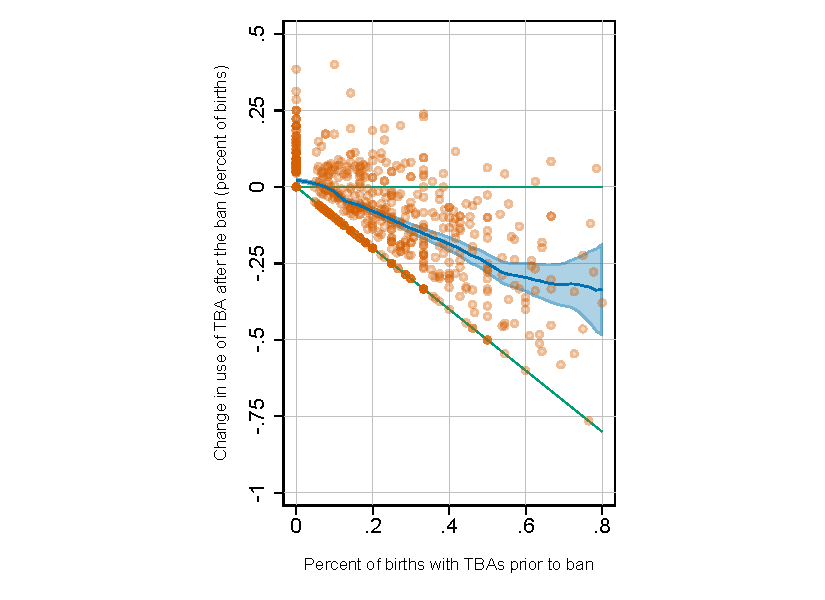
\includegraphics[height=5.2cm,trim = 3cm 0cm 3cm 0cm,clip]{fig/tba-change-scatter.pdf}};

	\node [oigreen,anchor=west,align=left,font=\small] (lbl1) at (5,2.5) {Post-ban mean must be positive};
	\draw [oigreen,thick,->] (lbl1.west) -- (3.75,2.25);
	\node [oigreen,anchor=west,align=left,font=\small] (lbl1) at (5,1.875) {$\Rightarrow$ Decline $\uparrow$ with pre-ban mean};
	
	\end{tikzpicture}
\end{center}


\end{frame}


%%%%%%%%%%%%%%%%%%%%%%%%%%%%%%%%%%%%%%%%%%%%%%%%%%%%%%%%%%%%%%%%%%%%%%%

\begin{frame}{Example:  Traditional Birth Attendants in Malawi}


\begin{center}
	\begin{tikzpicture}
	
	% blank canvas
	\only<handout>{\fill[fill=white,draw=white,ultra thin]
		(0,0) -- (11,0) -- (11,6) -- (0,6) -- cycle;}
	\only<beamer>{\fill[fill=white,draw=white,ultra thin]
		(0,0) -- (14,0) -- (14,6) -- (0,6) -- cycle;}
	\only<beamer>{\draw[draw=oiblue!60,fill=oiblue!10,opacity=0.5] (11,1) rectangle (14,5);}
	%\draw[step=1.0,gray!20,thin] (0,0) grid (11,6);	
	
	\node [anchor=north] (scatter) at (2.5,5.75) {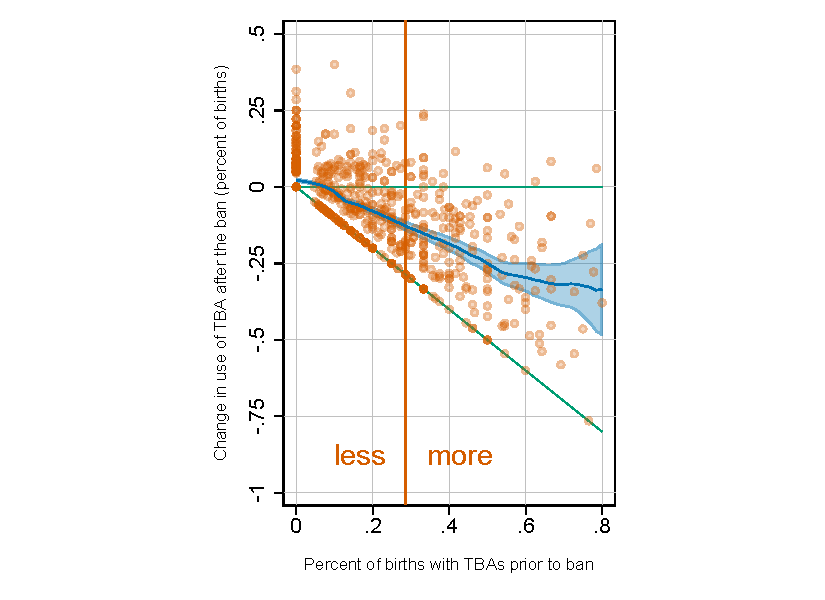
\includegraphics[height=5.2cm,trim = 3cm 0cm 3cm 0cm,clip]{fig/tba-change-scatter2.pdf}};
	
	\node [anchor=base west,align=left,font=\small,text width = 5.5cm] (text1) at (4.75,4.5) {Continous treatment $\Rightarrow$ two options:};
	\node [anchor=base west,align=left,font=\small] (text2) at ([xshift=0.5cm,yshift=-0.5cm]text1.south west) {\structure{$\bullet$} Discretize treatment};
	\node [anchor=base west,align=left,font=\small] (text3) at ([yshift=-0.5cm]text2.base west) {\structure{$\bullet$} Use continuous variable};

	\node [anchor=base west,align=left,font=\small,text width = 5.5cm] (text4) at ([xshift=-0.5cm,yshift=-0.75cm]text3.base west) {Both have pros and cons in terms of power, potential for mis-specification};
	\node [anchor=base west,align=left,font=\small] (text5) at ([xshift=0.5cm,yshift=-0.5cm]text4.south west) {\structure{$\bullet$} $\Delta Y$ specification $=$ bivariate OLS};
	
	\end{tikzpicture}
\end{center}


\end{frame}



%%%%%%%%%%%%%%%%%%%%%%%%%%%%%%%%%%%%%%%%%%%%%%%%%%%%%%%%%%%%%%%%%%%%%%%

\begin{frame}{Generalizing the Difference-in-Differences Framework}

\medskip
\textbf{Option 1:  partition sample into more/less treated}

\medskip
\begin{itemize}
	
	\item Treatment variable is a dummy for more-treated group
	
	\medskip
	\begin{itemize}
		
		\item Coefficient is difference in means between groups
		
	\end{itemize}

\pause
\item Estimand: difference in outcomes from increased treatment
	
\end{itemize}

\pause
\medskip
\medskip
\textbf{Option 2:  treatment as a continuous variable ($X_i$)}

\medskip
\begin{itemize}
	
	%\item $\beta_{OLS} = \frac{COV(X,Y)}{VAR(X)} = \frac{\sum_i Y_i \left(X_i - \bar{X} \right)}{\sum_i \left(X_i - \bar{X} \right)^2}$
	
	\item OLS coefficient is weighted sum of $Y_i$ values
	
	\item What is the estimand?  
	
\end{itemize}


\end{frame}




%%%%%%%%%%%%%%%%%%%%%%%%%%%%%%%%%%%%%%%%%%%%%%%%%%%%%%%%%%%%%%%%%%%%%%%

\begin{frame}<handout:0>{Treatment as a Continuous Variable}

\begin{center}
	\begin{tikzpicture}
	
	% blank canvas
	\only<handout>{\fill[fill=white,draw=white,ultra thin]
		(0,0) -- (11,0) -- (11,6) -- (0,6) -- cycle;}
	\only<beamer>{\fill[fill=white,draw=white,ultra thin]
		(0,0) -- (14,0) -- (14,6) -- (0,6) -- cycle;}
	\only<beamer>{\draw[draw=oiblue!60,fill=oiblue!10,opacity=0.5] (11,1) rectangle (14,5);}
	%\draw[step=1.0,gray!20,thin] (0,0) grid (11,6);	
	
	\node [anchor=north west,align=left] (text1) at (0.25,5.5) {OLS coefficient is weighted sum of $Y_i$ values:};
	\node [anchor=north,align=center] (text2) at ([yshift=-0.125cm]text1.south) {$\beta_{OLS} = \frac{COV(X,Y)}{VAR(X)} = \sum_i Y_i \left(\frac{ \left(X_i - \bar{X} \right)}{\sum_i \left(X_i - \bar{X} \right)^2} \right)$};
	
%	\node [oiblue,anchor=north,align=center,font=\small,text width=3.6cm] (text3) at ([xshift=-1.125cm,yshift=-0.75cm]text2.south east) {weights proportional to deviations from mean $X$};
%	\draw[oiblue,->] (text3.north) -- ([yshift=0.75cm]text3.north);
%	
%	\node [anchor=west,align=left] (text4) at (0.25,1.5) {In essence, the treatment group is $i$ with $X_i - \bar{X} > 0$};
	
	\end{tikzpicture}
\end{center}

\end{frame}



%%%%%%%%%%%%%%%%%%%%%%%%%%%%%%%%%%%%%%%%%%%%%%%%%%%%%%%%%%%%%%%%%%%%%%%

\begin{frame}<handout:0>{Treatment as a Continuous Variable}

\begin{center}
	\begin{tikzpicture}
	
	% blank canvas
	\only<handout>{\fill[fill=white,draw=white,ultra thin]
		(0,0) -- (11,0) -- (11,6) -- (0,6) -- cycle;}
	\only<beamer>{\fill[fill=white,draw=white,ultra thin]
		(0,0) -- (14,0) -- (14,6) -- (0,6) -- cycle;}
	\only<beamer>{\draw[draw=oiblue!60,fill=oiblue!10,opacity=0.5] (11,1) rectangle (14,5);}
	%\draw[step=1.0,gray!20,thin] (0,0) grid (11,6);	
	
	\node [anchor=north west,align=left] (text1) at (0.25,5.5) {OLS coefficient is weighted sum of $Y_i$ values:};
	\node [anchor=north,align=center] (text2) at ([yshift=-0.125cm]text1.south) {$\beta_{OLS} = \frac{COV(X,Y)}{VAR(X)} = \sum_i Y_i \left(\frac{ \left(X_i - \bar{X} \right)}{\sum_i \left(X_i - \bar{X} \right)^2} \right)$};
	
	\node [oiblue,anchor=north,align=center,font=\small,text width=3.6cm] (text3) at ([xshift=-1.125cm,yshift=-0.75cm]text2.south east) {weights proportional to deviations from mean $X$};
	\draw[oiblue,->] (text3.north) -- ([yshift=0.75cm]text3.north);
	
	%\node [anchor=west,align=left] (text4) at (0.25,1.5) {In essence, the treatment group is $i$ with $X_i - \bar{X} > 0$};
	
	\end{tikzpicture}
\end{center}

\end{frame}


%%%%%%%%%%%%%%%%%%%%%%%%%%%%%%%%%%%%%%%%%%%%%%%%%%%%%%%%%%%%%%%%%%%%%%%

\begin{frame}{Treatment as a Continuous Variable}

\begin{center}
	\begin{tikzpicture}
	
	% blank canvas
	\only<handout>{\fill[fill=white,draw=white,ultra thin]
		(0,0) -- (11,0) -- (11,6) -- (0,6) -- cycle;}
	\only<beamer>{\fill[fill=white,draw=white,ultra thin]
		(0,0) -- (14,0) -- (14,6) -- (0,6) -- cycle;}
	\only<beamer>{\draw[draw=oiblue!60,fill=oiblue!10,opacity=0.5] (11,1) rectangle (14,5);}
	%\draw[step=1.0,gray!20,thin] (0,0) grid (11,6);	
	
	\node [anchor=north west,align=left] (text1) at (0.25,5.5) {OLS coefficient is weighted sum of $Y_i$ values:};
	\node [anchor=north,align=center] (text2) at ([yshift=-0.125cm]text1.south) {$\beta_{OLS} = \frac{COV(X,Y)}{VAR(X)} = \sum_i Y_i \left(\frac{ \left(X_i - \bar{X} \right)}{\sum_i \left(X_i - \bar{X} \right)^2} \right)$};
	
	\node [oiblue,anchor=north,align=center,font=\small,text width=3.6cm] (text3) at ([xshift=-1.125cm,yshift=-0.75cm]text2.south east) {weights proportional to deviations from mean $X$};
	\draw[oiblue,->] (text3.north) -- ([yshift=0.75cm]text3.north);
	
	\node [anchor=west,align=left] (text4) at (0.25,1.5) {In essence, the treatment group is $i$ with $X_i - \bar{X} > 0$};
	
	\end{tikzpicture}
\end{center}

\end{frame}


%%%%%%%%%%%%%%%%%%%%%%%%%%%%%%%%%%%%%%%%%%%%%%%%%%%%%%%%%%%%%%%%%%%%%%%

\begin{frame}<handout:0>{The Dose-Response Relationship}

\begin{center}
	\begin{tikzpicture}
	
	% blank canvas
	\only<handout>{\fill[fill=white,draw=white,ultra thin]
		(0,0) -- (11,0) -- (11,6) -- (0,6) -- cycle;}
	\only<beamer>{\fill[fill=white,draw=white,ultra thin]
		(0,0) -- (14,0) -- (14,6) -- (0,6) -- cycle;}
	\only<beamer>{\draw[draw=oiblue!60,fill=oiblue!10,opacity=0.5] (11,1) rectangle (14,5);}
	%\draw[step=1.0,gray!20,thin] (0,0) grid (11,6);	
	
	\node [anchor=north west] (fig) at (0.25,5) {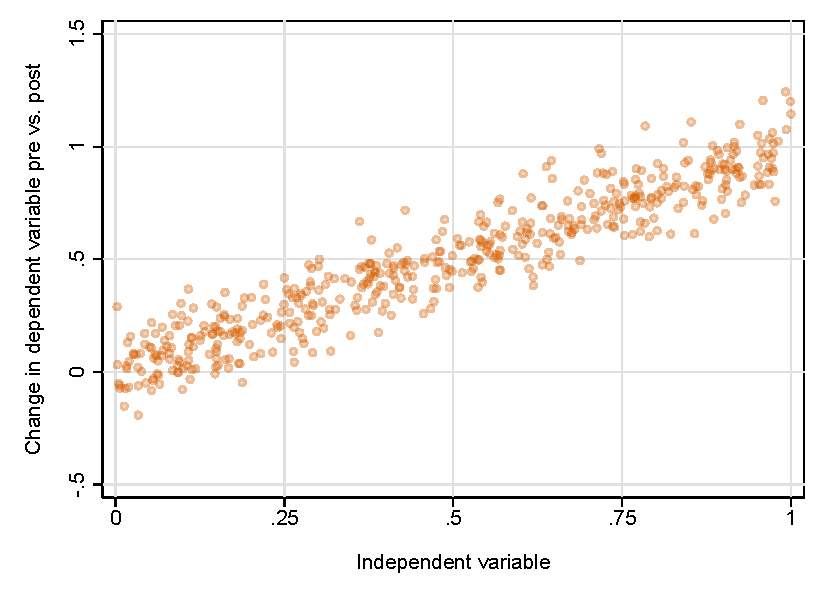
\includegraphics[width=6cm]{fig/linear-resp1.pdf}};
	
	\node [anchor=north west,font=\footnotesize] (text1) at (fig.north east) {Is dose-response linear?};
	
	\node [anchor=base west,font=\footnotesize] (text2) at ([xshift=0.25cm,yshift=-0.5cm]text1.base west) {$\Rightarrow$ If \textcolor{red}{yes}:  OLS FTW!};

	
	\end{tikzpicture}
\end{center}

\end{frame}


%%%%%%%%%%%%%%%%%%%%%%%%%%%%%%%%%%%%%%%%%%%%%%%%%%%%%%%%%%%%%%%%%%%%%%%

\begin{frame}{The Dose-Response Relationship}

\begin{center}
	\begin{tikzpicture}
	
	% blank canvas
	\only<handout>{\fill[fill=white,draw=white,ultra thin]
		(0,0) -- (11,0) -- (11,6) -- (0,6) -- cycle;}
	\only<beamer>{\fill[fill=white,draw=white,ultra thin]
		(0,0) -- (14,0) -- (14,6) -- (0,6) -- cycle;}
	\only<beamer>{\draw[draw=oiblue!60,fill=oiblue!10,opacity=0.5] (11,1) rectangle (14,5);}
	%\draw[step=1.0,gray!20,thin] (0,0) grid (11,6);	
	
	\node [anchor=north west] (fig) at (0.25,5) {\includegraphics[width=6cm]{fig/linear-resp2.pdf}};
	
	\node [anchor=north west,font=\footnotesize] (text1) at (fig.north east) {Is dose-response linear?};
	
	\node [anchor=base west,font=\footnotesize] (text2) at ([xshift=0.25cm,yshift=-0.5cm]text1.base west) {$\Rightarrow$ If \textcolor{red}{yes}:  OLS FTW!};

	\node [anchor=base west,font=\footnotesize] (text3) at ([xshift=-0.25cm,yshift=-0.75cm]text2.base west) {$\beta_{OLS} = $ weighted sum of $Y_i$s};	
	
	\node [anchor=base west,font=\footnotesize] (text4) at ([xshift=0.25cm,yshift=-0.5cm]text3.base west) {\structure{$\bullet$} Negative weights $\Leftrightarrow X_i < \bar{X}$ };
	\node [anchor=base west,font=\footnotesize] (text5) at ([xshift=0cm,yshift=-0.5cm]text4.base west) {\structure{$\bullet$} Proportional to $| X_i - \bar{X} |$ };
	
	\end{tikzpicture}
\end{center}

\end{frame}



%%%%%%%%%%%%%%%%%%%%%%%%%%%%%%%%%%%%%%%%%%%%%%%%%%%%%%%%%%%%%%%%%%%%%%%

\begin{frame}{The Dose-Response Relationship}

\begin{center}
	\begin{tikzpicture}
	
	% blank canvas
	\only<handout>{\fill[fill=white,draw=white,ultra thin]
		(0,0) -- (11,0) -- (11,6) -- (0,6) -- cycle;}
	\only<beamer>{\fill[fill=white,draw=white,ultra thin]
		(0,0) -- (14,0) -- (14,6) -- (0,6) -- cycle;}
	\only<beamer>{\draw[draw=oiblue!60,fill=oiblue!10,opacity=0.5] (11,1) rectangle (14,5);}
	%\draw[step=1.0,gray!20,thin] (0,0) grid (11,6);	
	
	\node [anchor=north west] (fig) at (0.25,5) {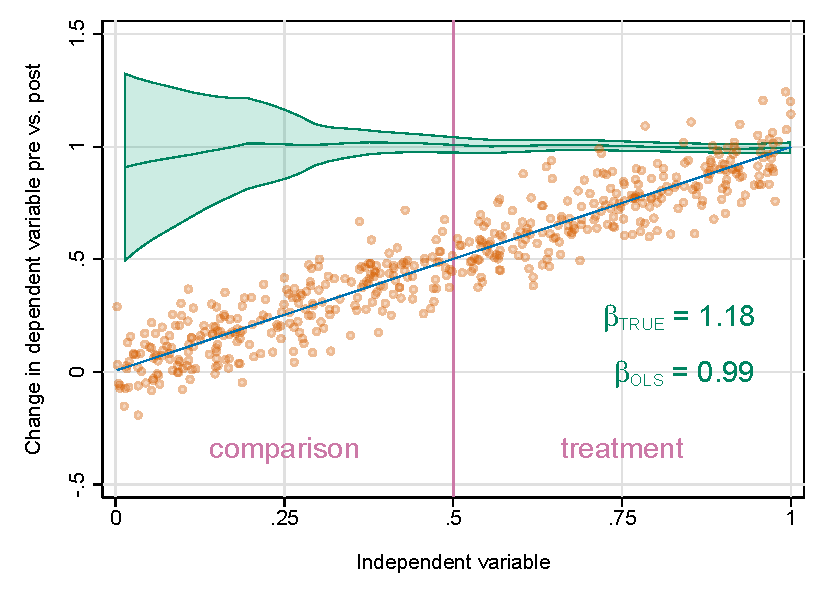
\includegraphics[width=6cm]{fig/linear-resp-explain.pdf}};
	
	\node [anchor=north west,font=\footnotesize] (text1) at (fig.north east) {Is dose-response linear?};
	
	\node [anchor=base west,font=\footnotesize] (text2) at ([xshift=0.25cm,yshift=-0.5cm]text1.base west) {$\Rightarrow$ If \textcolor{red}{yes}:  OLS FTW!};
	
	\node [anchor=base west,font=\footnotesize] (text3) at ([xshift=-0.25cm,yshift=-0.75cm]text2.base west) {$\beta_{OLS} = $ weighted sum of $Y_i$s};	
	
	\node [anchor=base west,font=\footnotesize] (text4) at ([xshift=0.25cm,yshift=-0.5cm]text3.base west) {\structure{$\bullet$} Negative weights $\Leftrightarrow X_i < \bar{X}$ };
	\node [anchor=base west,font=\footnotesize] (text5) at ([xshift=0cm,yshift=-0.5cm]text4.base west) {\structure{$\bullet$} Proportional to $| X_i - \bar{X} |$ };
	
	\node [anchor=base west,font=\footnotesize,text width = 4cm] (text6) at ([xshift=-0.25cm,yshift=-0.75cm]text5.base west) {OLS is specified correctly, \\
		 maximizes statisticaly power};
	
	\end{tikzpicture}
\end{center}

\end{frame}


%%%%%%%%%%%%%%%%%%%%%%%%%%%%%%%%%%%%%%%%%%%%%%%%%%%%%%%%%%%%%%%%%%%%%%%

\begin{frame}<handout:0>{The Dose-Response Relationship}

\begin{center}
	\begin{tikzpicture}
	
	% blank canvas
	\only<handout>{\fill[fill=white,draw=white,ultra thin]
		(0,0) -- (11,0) -- (11,6) -- (0,6) -- cycle;}
	\only<beamer>{\fill[fill=white,draw=white,ultra thin]
		(0,0) -- (14,0) -- (14,6) -- (0,6) -- cycle;}
	\only<beamer>{\draw[draw=oiblue!60,fill=oiblue!10,opacity=0.5] (11,1) rectangle (14,5);}
	%\draw[step=1.0,gray!20,thin] (0,0) grid (11,6);	
	
	\node [anchor=north west] (fig) at (0.25,5) {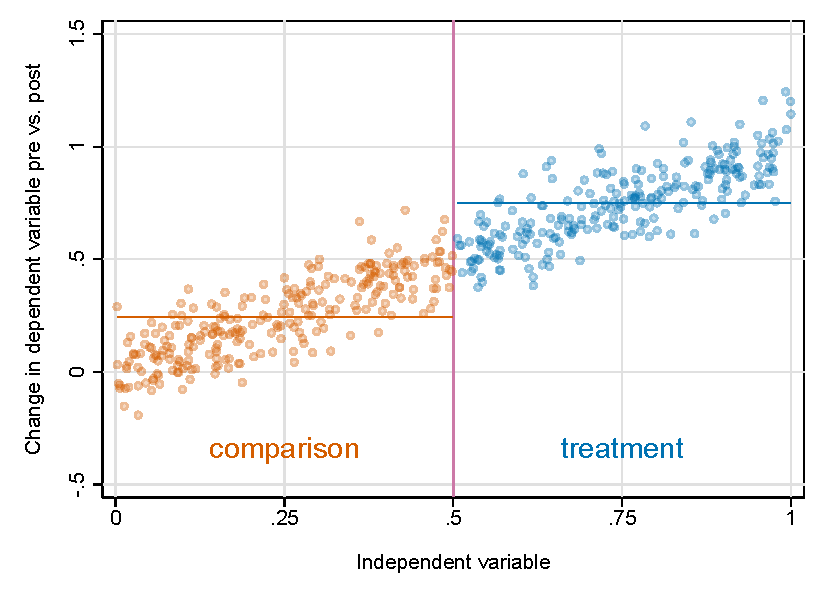
\includegraphics[width=6cm]{fig/linear-resp3.pdf}};
	
	\node [anchor=north west,font=\footnotesize] (text1) at (fig.north east) {When we discretize $X_i$:};
	
	\node [anchor=base west,font=\footnotesize] (text2) at ([xshift=0.25cm,yshift=-0.5cm]text1.base west) {$\Rightarrow$ Estimating impact of $\Delta X_i$};
	
	\end{tikzpicture}
\end{center}

\end{frame}



%%%%%%%%%%%%%%%%%%%%%%%%%%%%%%%%%%%%%%%%%%%%%%%%%%%%%%%%%%%%%%%%%%%%%%%

\begin{frame}{The Dose-Response Relationship}

\begin{center}
	\begin{tikzpicture}
	
	% blank canvas
	\only<handout>{\fill[fill=white,draw=white,ultra thin]
		(0,0) -- (11,0) -- (11,6) -- (0,6) -- cycle;}
	\only<beamer>{\fill[fill=white,draw=white,ultra thin]
		(0,0) -- (14,0) -- (14,6) -- (0,6) -- cycle;}
	\only<beamer>{\draw[draw=oiblue!60,fill=oiblue!10,opacity=0.5] (11,1) rectangle (14,5);}
	%\draw[step=1.0,gray!20,thin] (0,0) grid (11,6);	
	
	\node [anchor=north west] (fig) at (0.25,5) {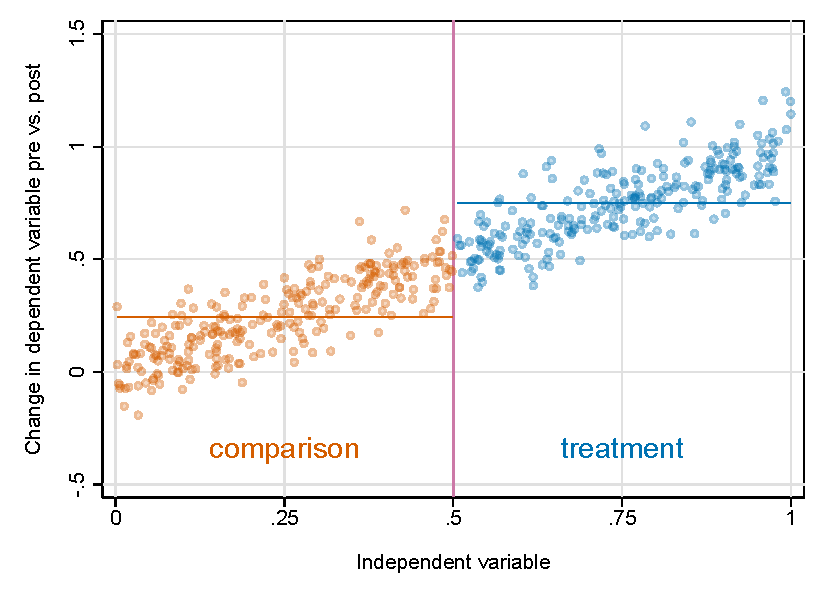
\includegraphics[width=6cm]{fig/linear-resp3.pdf}};
	
	\node [anchor=north west,font=\footnotesize] (text1) at (fig.north east) {When we discretize $X_i$:};
	
	\node [anchor=base west,font=\footnotesize] (text2) at ([xshift=0.25cm,yshift=-0.5cm]text1.base west) {$\Rightarrow$ Estimating impact of $\Delta X_i$};
	
		\node [anchor=base west,font=\footnotesize] (text3) at ([xshift=-0.25cm,yshift=-0.75cm]text2.base west) {$\beta_{OLS} = $ difference in means};	
		
	%	\node [anchor=base west,font=\footnotesize] (text4) at ([xshift=0.25cm,yshift=-0.5cm]text3.base west) {\structure{$\bullet$} Negative weights $\Leftrightarrow X_i < \bar{X}$ };
	%	\node [anchor=base west,font=\footnotesize] (text5) at ([xshift=0cm,yshift=-0.5cm]text4.base west) {\structure{$\bullet$} Proportional to $| X_i - \bar{X} |$ };
	%	
	%	\node [anchor=base west,font=\footnotesize,text width = 4cm] (text6) at ([xshift=-0.25cm,yshift=-0.625cm]text5.base west) {OLS is specified correctly, \\
	%		maximizes statisticaly power};
	
	\end{tikzpicture}
\end{center}

\end{frame}



%%%%%%%%%%%%%%%%%%%%%%%%%%%%%%%%%%%%%%%%%%%%%%%%%%%%%%%%%%%%%%%%%%%%%%%

\begin{frame}{The Dose-Response Relationship}

\begin{center}
	\begin{tikzpicture}
	
	% blank canvas
	\only<handout>{\fill[fill=white,draw=white,ultra thin]
		(0,0) -- (11,0) -- (11,6) -- (0,6) -- cycle;}
	\only<beamer>{\fill[fill=white,draw=white,ultra thin]
		(0,0) -- (14,0) -- (14,6) -- (0,6) -- cycle;}
	\only<beamer>{\draw[draw=oiblue!60,fill=oiblue!10,opacity=0.5] (11,1) rectangle (14,5);}
	%\draw[step=1.0,gray!20,thin] (0,0) grid (11,6);	
	
	\node [anchor=north west] (fig) at (0.25,5) {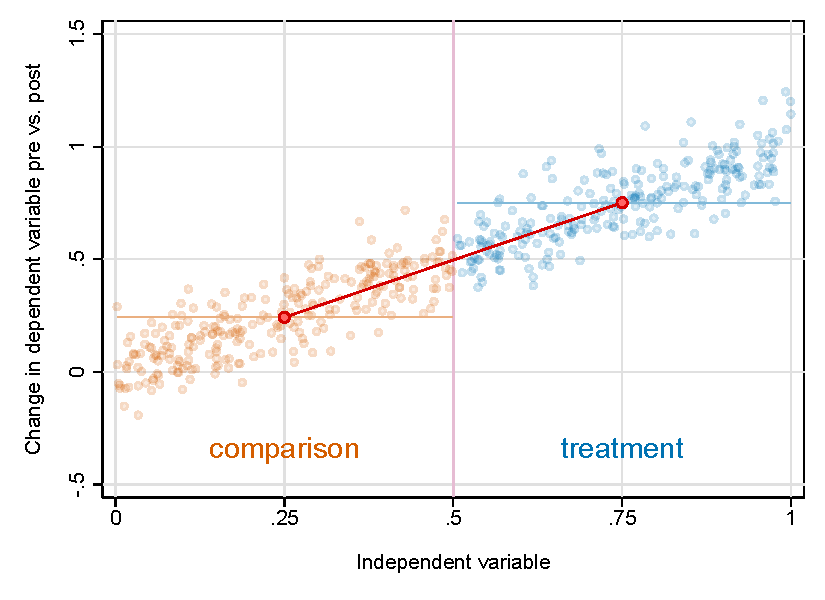
\includegraphics[width=6cm]{fig/linear-resp4.pdf}};
	
	\node [anchor=north west,font=\footnotesize] (text1) at (fig.north east) {When we discretize $X_i$:};
	
	\node [anchor=base west,font=\footnotesize] (text2) at ([xshift=0.25cm,yshift=-0.5cm]text1.base west) {$\Rightarrow$ Estimating impact of $\Delta X_i$};
	
	\node [anchor=base west,font=\footnotesize] (text3) at ([xshift=-0.25cm,yshift=-0.75cm]text2.base west) {$\beta_{OLS} = $ difference in means};	
	
	\node [red,anchor=base west,font=\footnotesize,text width = 4cm] (text4) at ([xshift=0cm,yshift=-0.75cm]text3.base west) {$(\bar{X}_C,\bar{Y}_C)$ to $(\bar{X}_T,\bar{Y}_T)$ line \\
		captures linear relationship};
	\draw[red,thick,->] (text4.west) -- (4.375,3.125);
	
	\end{tikzpicture}
\end{center}

\end{frame}



%%%%%%%%%%%%%%%%%%%%%%%%%%%%%%%%%%%%%%%%%%%%%%%%%%%%%%%%%%%%%%%%%%%%%%%

\begin{frame}{The Dose-Response Relationship}

\begin{center}
	\begin{tikzpicture}
	
	% blank canvas
	\only<handout>{\fill[fill=white,draw=white,ultra thin]
		(0,0) -- (11,0) -- (11,6) -- (0,6) -- cycle;}
	\only<beamer>{\fill[fill=white,draw=white,ultra thin]
		(0,0) -- (14,0) -- (14,6) -- (0,6) -- cycle;}
	\only<beamer>{\draw[draw=oiblue!60,fill=oiblue!10,opacity=0.5] (11,1) rectangle (14,5);}
	%\draw[step=1.0,gray!20,thin] (0,0) grid (11,6);	
	
	\node [anchor=north west] (fig) at (0.25,5) {\includegraphics[width=6cm]{fig/linear-resp5.pdf}};
	
	\node [anchor=north west,font=\footnotesize] (text1) at (fig.north east) {When we discretize $X_i$:};
	
	\node [anchor=base west,font=\footnotesize] (text2) at ([xshift=0.25cm,yshift=-0.5cm]text1.base west) {$\Rightarrow$ Estimating impact of $\Delta X_i$};
	
	\node [anchor=base west,font=\footnotesize] (text3) at ([xshift=-0.25cm,yshift=-0.75cm]text2.base west) {$\beta_{OLS} = $ difference in means};	
	
	\node [anchor=base west,font=\footnotesize,text width = 4cm] (text4) at ([xshift=0cm,yshift=-0.75cm]text3.base west) {$(\bar{X}_C,\bar{Y}_C)$ to $(\bar{X}_T,\bar{Y}_T)$ line \\
		captures linear relationship};
	
	\node [anchor=base west,font=\footnotesize,text width = 4cm] (text5) at ([xshift=0cm,yshift=-1cm]text4.base west) {Not what we get from a \\
		dummy for ``more treated''};
	
	\node [red,anchor=base west,font=\footnotesize] (text6) at ([xshift=0.25cm,yshift=-0.875cm]text5.base west) {$\Rightarrow \beta_{OLS}$ biased toward 0?};

	
	\end{tikzpicture}
\end{center}

\end{frame}



%%%%%%%%%%%%%%%%%%%%%%%%%%%%%%%%%%%%%%%%%%%%%%%%%%%%%%%%%%%%%%%%%%%%%%%

\begin{frame}<handout:0>{When Dose-Response Relationship is Not Linear}

\begin{center}
	\begin{tikzpicture}
	
	% blank canvas
	\only<handout>{\fill[fill=white,draw=white,ultra thin]
		(0,0) -- (11,0) -- (11,6) -- (0,6) -- cycle;}
	\only<beamer>{\fill[fill=white,draw=white,ultra thin]
		(0,0) -- (14,0) -- (14,6) -- (0,6) -- cycle;}
	\only<beamer>{\draw[draw=oiblue!60,fill=oiblue!10,opacity=0.5] (11,1) rectangle (14,5);}
	%\draw[step=1.0,gray!20,thin] (0,0) grid (11,6);	
	
	\node [anchor=north west] (fig) at (0.25,5) {\includegraphics[width=6cm]{fig/concave-resp1.pdf}};
	
	\node [anchor=north west,font=\footnotesize] (text1) at (fig.north east) {Continuous treatment variable};
	
	\node [anchor=base west,font=\footnotesize] (text2) at ([xshift=0cm,yshift=-0.5cm]text1.base west) {$ + $ non-linear dose-response};
	
	\node [anchor=base west,font=\footnotesize] (text3) at ([xshift=0cm,yshift=-0.5cm]text2.base west) {$ = $ big trouble};	
	
	\end{tikzpicture}
\end{center}

\end{frame}



%%%%%%%%%%%%%%%%%%%%%%%%%%%%%%%%%%%%%%%%%%%%%%%%%%%%%%%%%%%%%%%%%%%%%%%

\begin{frame}{When Dose-Response Relationship is Not Linear}

\begin{center}
	\begin{tikzpicture}
	
	% blank canvas
	\only<handout>{\fill[fill=white,draw=white,ultra thin]
		(0,0) -- (11,0) -- (11,6) -- (0,6) -- cycle;}
	\only<beamer>{\fill[fill=white,draw=white,ultra thin]
		(0,0) -- (14,0) -- (14,6) -- (0,6) -- cycle;}
	\only<beamer>{\draw[draw=oiblue!60,fill=oiblue!10,opacity=0.5] (11,1) rectangle (14,5);}
	%\draw[step=1.0,gray!20,thin] (0,0) grid (11,6);	
	
	\node [anchor=north west] (fig) at (0.25,5) {\includegraphics[width=6cm]{fig/concave-resp2.pdf}};
	
	\node [anchor=north west,font=\footnotesize] (text1) at (fig.north east) {Continuous treatment variable};
	
	\node [anchor=base west,font=\footnotesize] (text2) at ([xshift=0cm,yshift=-0.5cm]text1.base west) {$ + $ non-linear dose-response};
	
	\node [anchor=base west,font=\footnotesize] (text3) at ([xshift=0cm,yshift=-0.5cm]text2.base west) {$ = $ big trouble};	
	
		\node [anchor=base west,font=\footnotesize,text width = 4cm] (text4) at ([xshift=0cm,yshift=-0.75cm]text3.base west) {Treatent effect when $X_i>0$};
	
	\node [anchor=base west,font=\footnotesize,text width = 4cm] (text5) at ([xshift=0.25cm,yshift=-0.5cm]text4.base west) {\structure{$\bullet$} Not linear in $X_i$};
		
	\node [anchor=base west,font=\footnotesize] (text6) at ([xshift=-0.25cm,yshift=-0.75cm]text5.base west) {$\Rightarrow \beta_{OLS}$ not ATE};
	
	
	\end{tikzpicture}
\end{center}

\end{frame}



%%%%%%%%%%%%%%%%%%%%%%%%%%%%%%%%%%%%%%%%%%%%%%%%%%%%%%%%%%%%%%%%%%%%%%%

\begin{frame}<handout:0>{When Dose-Response Relationship is Not Linear}

\begin{center}
	\begin{tikzpicture}
	
	% blank canvas
	\only<handout>{\fill[fill=white,draw=white,ultra thin]
		(0,0) -- (11,0) -- (11,6) -- (0,6) -- cycle;}
	\only<beamer>{\fill[fill=white,draw=white,ultra thin]
		(0,0) -- (14,0) -- (14,6) -- (0,6) -- cycle;}
	\only<beamer>{\draw[draw=oiblue!60,fill=oiblue!10,opacity=0.5] (11,1) rectangle (14,5);}
	%\draw[step=1.0,gray!20,thin] (0,0) grid (11,6);	
	
	\node [anchor=north west] (fig) at (0.25,5) {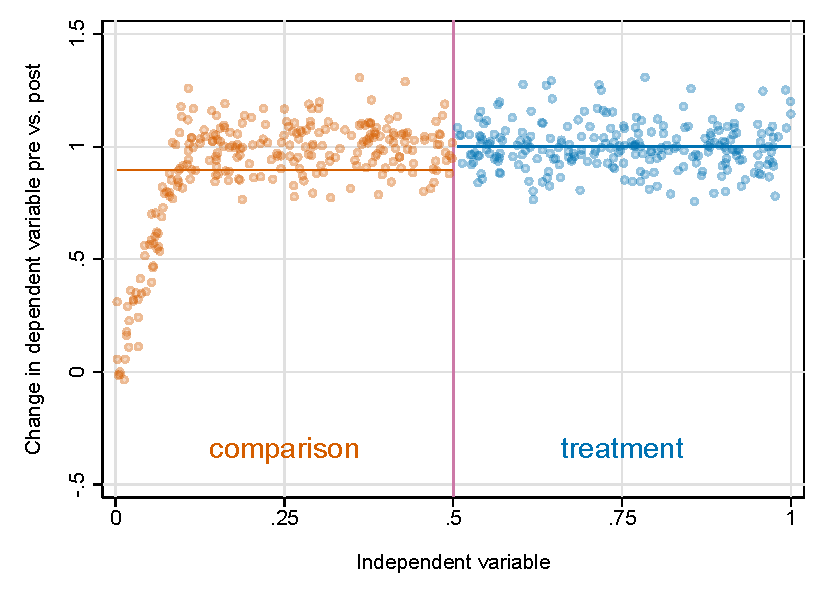
\includegraphics[width=6cm]{fig/concave-resp3.pdf}};
	
	\node [anchor=north west,font=\footnotesize] (text1) at (fig.north east) {Binary treatment variable:};
	
	\node [anchor=base west,font=\footnotesize] (text2) at ([xshift=0.25cm,yshift=-0.625cm]text1.base west) {\structure{$\bullet$} Small difference in means};
	
	\node [anchor=base west,font=\footnotesize] (text3) at ([xshift=0cm,yshift=-0.5cm]text2.base west) {\structure{$\bullet$} $\Delta \bar{Y}_T$, $\Delta \bar{Y}_C$ similar};	
	
	\node [anchor=base west,font=\footnotesize,text width = 4cm] (text4) at ([xshift=0cm,yshift=-0.5cm]text3.base west) {\structure{$\bullet$} Treatment effect in  $\Delta \bar{Y}_C$};
	
%	\node [anchor=base west,font=\footnotesize,text width = 4cm] (text5) at ([xshift=0.25cm,yshift=-0.5cm]text4.base west) {\structure{$\bullet$} Not linear in $X_i$};
%	
%	\node [anchor=base west,font=\footnotesize] (text6) at ([xshift=-0.25cm,yshift=-0.75cm]text5.base west) {$\Rightarrow \beta_{OLS}$ not ATE};
	
	
	\end{tikzpicture}
\end{center}

\end{frame}



%%%%%%%%%%%%%%%%%%%%%%%%%%%%%%%%%%%%%%%%%%%%%%%%%%%%%%%%%%%%%%%%%%%%%%%

\begin{frame}{When Dose-Response Relationship is Not Linear}

\begin{center}
	\begin{tikzpicture}
	
	% blank canvas
	\only<handout>{\fill[fill=white,draw=white,ultra thin]
		(0,0) -- (11,0) -- (11,6) -- (0,6) -- cycle;}
	\only<beamer>{\fill[fill=white,draw=white,ultra thin]
		(0,0) -- (14,0) -- (14,6) -- (0,6) -- cycle;}
	\only<beamer>{\draw[draw=oiblue!60,fill=oiblue!10,opacity=0.5] (11,1) rectangle (14,5);}
	%\draw[step=1.0,gray!20,thin] (0,0) grid (11,6);	
	
	\node [anchor=north west] (fig) at (0.25,5) {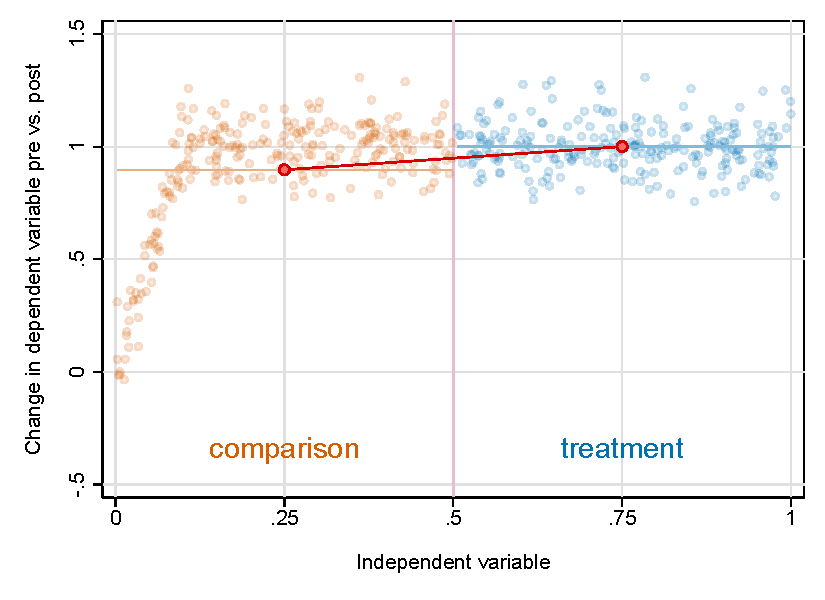
\includegraphics[width=6cm]{fig/concave-resp4.pdf}};
	
	\node [anchor=north west,font=\footnotesize] (text1) at (fig.north east) {Binary treatment variable:};
	
	\node [anchor=base west,font=\footnotesize] (text2) at ([xshift=0.25cm,yshift=-0.625cm]text1.base west) {\structure{$\bullet$} Small difference in means};
	
	\node [anchor=base west,font=\footnotesize] (text3) at ([xshift=0cm,yshift=-0.5cm]text2.base west) {\structure{$\bullet$} $\Delta \bar{Y}_T$, $\Delta \bar{Y}_C$ similar};	
	
	\node [anchor=base west,font=\footnotesize,text width = 4cm] (text4) at ([xshift=0cm,yshift=-0.5cm]text3.base west) {\structure{$\bullet$} Treatment effect in  $\Delta \bar{Y}_C$};
	
		\node [anchor=base west,font=\footnotesize,text width = 4cm] (text5) at ([xshift=-0.25cm,yshift=-0.75cm]text4.base west) {$\beta_{OLS}$ unbiased estimate of \\ impact of $\bar{X}_C$ to $\bar{X}_T$ shift};
		
		\node [anchor=base west,font=\footnotesize] (text6) at ([xshift=0cm,yshift=-0.875cm]text5.base west) {$\Rightarrow$ Conservative approach};
	
	
	\end{tikzpicture}
\end{center}

\end{frame}



%%%%%%%%%%%%%%%%%%%%%%%%%%%%%%%%%%%%%%%%%%%%%%%%%%%%%%%%%%%%%%%%%%%%%%%

\begin{frame}{When Dose-Response Relationship is Not Linear}

\begin{center}
	\begin{tikzpicture}
	
	% blank canvas
	\only<handout>{\fill[fill=white,draw=white,ultra thin]
		(0,0) -- (11,0) -- (11,6) -- (0,6) -- cycle;}
	\only<beamer>{\fill[fill=white,draw=white,ultra thin]
		(0,0) -- (14,0) -- (14,6) -- (0,6) -- cycle;}
	\only<beamer>{\draw[draw=oiblue!60,fill=oiblue!10,opacity=0.5] (11,1) rectangle (14,5);}
	%\draw[step=1.0,gray!20,thin] (0,0) grid (11,6);	
	
	\node [anchor=north west] (fig) at (0.25,5) {\includegraphics[width=6cm]{fig/concave-resp5.pdf}};
	
	\node [anchor=north west,font=\footnotesize] (text1) at (fig.north east) {Binary treatment variable:};
	
	\node [anchor=base west,font=\footnotesize] (text2) at ([xshift=0.25cm,yshift=-0.625cm]text1.base west) {\structure{$\bullet$} Small difference in means};
	
	\node [anchor=base west,font=\footnotesize] (text3) at ([xshift=0cm,yshift=-0.5cm]text2.base west) {\structure{$\bullet$} $\Delta \bar{Y}_T$, $\Delta \bar{Y}_C$ similar};	
	
	\node [anchor=base west,font=\footnotesize,text width = 4cm] (text4) at ([xshift=0cm,yshift=-0.5cm]text3.base west) {\structure{$\bullet$} Treatment effect in  $\Delta \bar{Y}_C$};
	
	\node [anchor=base west,font=\footnotesize,text width = 4cm] (text5) at ([xshift=-0.25cm,yshift=-0.75cm]text4.base west) {$\beta_{OLS}$ unbiased estimate of \\ impact of $\bar{X}_C$ to $\bar{X}_T$ shift};
	
	\node [anchor=base west,font=\footnotesize] (text6) at ([xshift=0cm,yshift=-0.875cm]text5.base west) {$\Rightarrow$ Conservative approach};
	
	
	\end{tikzpicture}
\end{center}

\end{frame}




%%%%%%%%%%%%%%%%%%%%%%%%%%%%%%%%%%%%%%%%%%%%%%%%%%%%%%%%%%%%%%%%%%%%%%%

\begin{frame}{Flavors of Diff-in-Diff:  Summary}

\medskip
\textbf{Treatment is fundamentally binary:  us a treatment dummy}

\medskip
\begin{itemize}
	
	\item Examples:  Chicago police reform, NJ minimum wage
	
	\item Clear how to interpret, unbiased (w/ common trends)
	
\end{itemize}

\medskip
\textbf{Treatment is fundamentally continuous:  }

\medskip
\begin{itemize}
	
	\item \textcolor{red}{Use a treatment dummy (discretize treatment)}
	
	\medskip
	\begin{itemize}
		
		\item Clear how to interpret coefficient, nature of estimand
		
		\item Understates impacts when ``comparison'' group is impacted 
		
	\end{itemize}
	
	\item \textcolor{red}{Use continuous variation in treatment}
	
	\medskip
	\begin{itemize}
		
		\item Increases power when dose-response relationship close to linear
		
		\item May give you garbage when dose-response non-linear
		
%		\medskip
%		\begin{itemize}
%			
%			\item Always make a graph!
%			
%		\end{itemize}
		
	\end{itemize}
	
\end{itemize}


\end{frame}




%%%%%%%%%%%%%%%%%%%%%%%%%%%%%%%%%%%%%%%%%%%%%%%%%%%%%%%%%%%%%%%%%%%%%%%

\begin{frame}{Dose-Response Relationship in Malawi TBAs Paper}

\begin{center}
	\begin{tikzpicture}
	
	% blank canvas
	\only<handout>{\fill[fill=white,draw=white,ultra thin]
		(0,0) -- (11,0) -- (11,6) -- (0,6) -- cycle;}
	\only<beamer>{\fill[fill=white,draw=white,ultra thin]
		(0,0) -- (14,0) -- (14,6) -- (0,6) -- cycle;}
	\only<beamer>{\draw[draw=oiblue!60,fill=oiblue!10,opacity=0.5] (11,1) rectangle (14,5);}
	%\draw[step=1.0,gray!20,thin] (0,0) grid (11,6);	
	
	\node [anchor=north west] (fig) at (0.25,5.75) {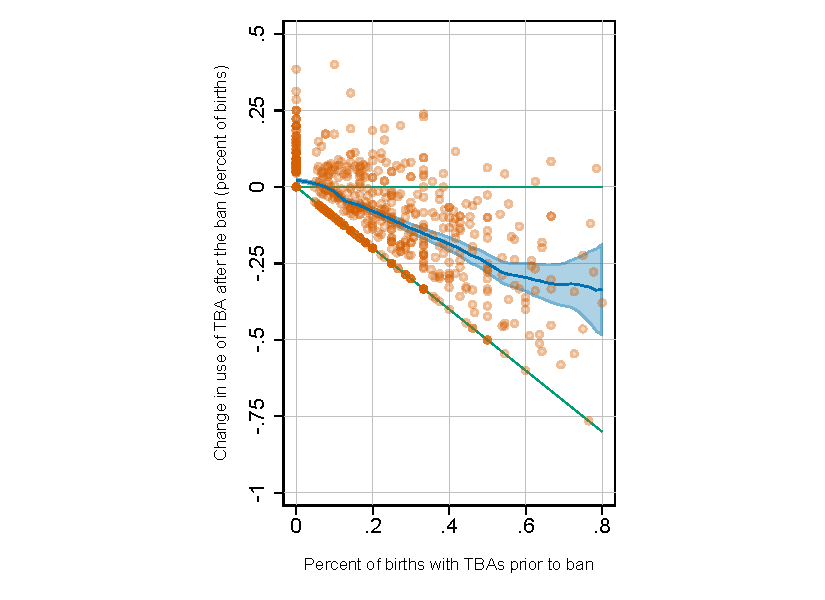
\includegraphics[height=5.2cm,trim = 3cm 0cm 3cm 0cm,clip]{fig/tba-change-scatter.pdf}};
	\node [anchor=north west] (fig2) at (fig.north east) {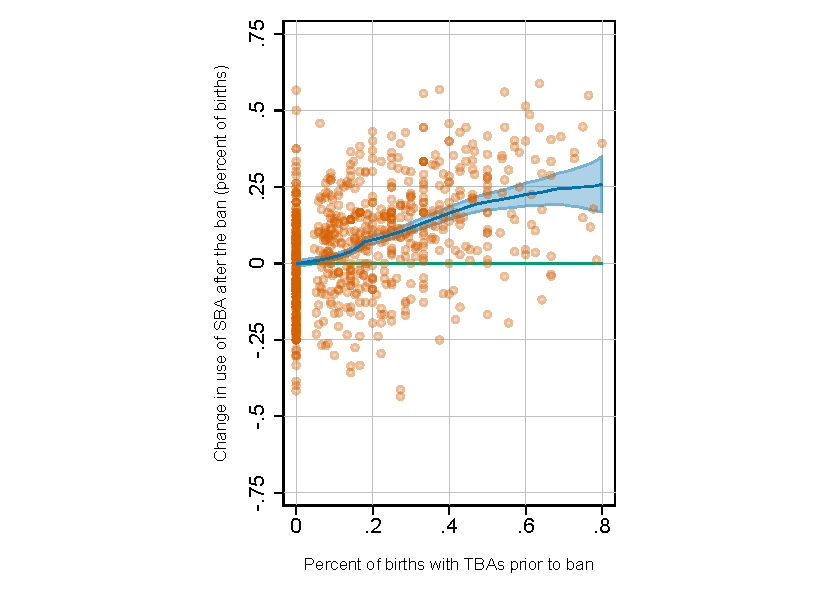
\includegraphics[height=5.2cm,trim = 3cm 0cm 3cm 0cm,clip]{fig/sba-change-scatter.pdf}};	

	
	\end{tikzpicture}
\end{center}

\end{frame}



%%%%%%%%%%%%%%%%%%%%%%%%%%%%%%%%%%%%%%%%%%%%%%%%%%%%%%%%%%%%%%%%%%%%%%%

\begin{frame}{Dose-Response Relationship in School Construction Paper}

\begin{center}
	\begin{tikzpicture}
	
	% blank canvas
	\only<handout>{\fill[fill=white,draw=white,ultra thin]
		(0,0) -- (11,0) -- (11,6) -- (0,6) -- cycle;}
	\only<beamer>{\fill[fill=white,draw=white,ultra thin]
		(0,0) -- (14,0) -- (14,6) -- (0,6) -- cycle;}
	\only<beamer>{\draw[draw=oiblue!60,fill=oiblue!10,opacity=0.5] (11,1) rectangle (14,5);}
	%\draw[step=1.0,gray!20,thin] (0,0) grid (11,6);	
	
	\node [anchor=north] (fig) at (5,4.75) {\includegraphics[width=8cm]{img/Duflo-NBER-fig.pdf}};
	\textcolor{gray}{\tiny{source:  Duflo (2000)}}

	\end{tikzpicture}
\end{center}

\end{frame}






%%%%%%%%%%%%%%%%%%%%%%%%%%%%%%%%%%%%%%%%%%%%%%%%%%%%%%%%%%%%%%%%%%%%%%%%%%%

%\begin{frame}<handout:0>[bg,plain]
\begin{frame}[plain]

\only<beamer>{\begin{adjustwidth}{0cm}{-4cm}}
	
	\begin{center}
		
		\Large{Fixed Effects}
		
	\end{center}
	
	\only<beamer>{\end{adjustwidth}}
\end{frame}



%%%%%%%%%%%%%%%%%%%%%%%%%%%%%%%%%%%%%%%%%%%%%%%%%%%%%%%%%%%%%%%%%%%%%%%%%%%%%%%

\begin{frame}{Generalized Diff-in-Diff with Fixed Effects}

\medskip
Widely used panel data diff-in-diff specification:  
\begin{small}
	\begin{equation*}
	Y_{i,t} = \alpha + \gamma D_{i,t} + \textcolor{black}{\delta} \left( D_{i,t} \times Post_t \right) + \textcolor{black}{\nu_t}  + \varepsilon_{i,t}
	\end{equation*}
\end{small}

\vspace{-0.32cm}

%\pause
where:

\medskip
\begin{itemize}
	
	\item $D_{i,t} = $ treatment dummy (could be continuous variable)
	
	\item \textcolor{black}{$\delta = $ diff-in-diff estimate of treatment effect}
	
	\item \textcolor{black}{$\nu_t = $ time-period fixed effects}

	
\end{itemize}

\end{frame}


%%%%%%%%%%%%%%%%%%%%%%%%%%%%%%%%%%%%%%%%%%%%%%%%%%%%%%%%%%%%%%%%%%%%%%%%%%%%%%%

\begin{frame}<handout:0>{Generalized Diff-in-Diff with Fixed Effects}

\medskip
Widely used panel data diff-in-diff specification:  
\begin{small}
	\begin{equation*}
	Y_{i,t} = \alpha + \gamma D_{i,t} + \textcolor{red}{\delta} \left( D_{i,t} \times Post_t \right) + \textcolor{black}{\nu_t}  + \varepsilon_{i,t}
	\end{equation*}
\end{small}

\vspace{-0.32cm}

%\pause
where:

\medskip
\begin{itemize}
	
	\item $D_{i,t} = $ treatment dummy (could be continuous variable)
	
	\item \textcolor{red}{$\delta = $ diff-in-diff estimate of treatment effect}
	
	\item \textcolor{black}{$\nu_t = $ time-period fixed effects}
	
	
\end{itemize}

\end{frame}


%%%%%%%%%%%%%%%%%%%%%%%%%%%%%%%%%%%%%%%%%%%%%%%%%%%%%%%%%%%%%%%%%%%%%%%%%%%%%%%

\begin{frame}<handout:0>{Generalized Diff-in-Diff with Fixed Effects}

\medskip
Widely used panel data diff-in-diff specification:  
\begin{small}
	\begin{equation*}
	Y_{i,t} = \alpha + \gamma D_{i,t} + \textcolor{black}{\delta} \left( D_{i,t} \times Post_t \right) + \textcolor{red}{\nu_t}  + \varepsilon_{i,t}
	\end{equation*}
\end{small}

\vspace{-0.32cm}

%\pause
where:

\medskip
\begin{itemize}
	
	\item $D_{i,t} = $ treatment dummy (could be continuous variable)
	
	\item \textcolor{black}{$\delta = $ diff-in-diff estimate of treatment effect}
	
	\item \textcolor{red}{$\nu_t = $ time-period fixed effects}
	
	
\end{itemize}

\end{frame}



%%%%%%%%%%%%%%%%%%%%%%%%%%%%%%%%%%%%%%%%%%%%%%%%%%%%%%%%%%%%%%%%%%%%%%%%%%%%%%%

\begin{frame}{What Do Fixed Effects Do?}

\begin{center}
	\begin{tikzpicture}
	
	% blank canvas
	\only<handout>{\fill[fill=white,draw=white,ultra thin]
		(0,0) -- (11,0) -- (11,6) -- (0,6) -- cycle;}
	\only<beamer>{\fill[fill=white,draw=white,ultra thin]
		(0,0) -- (14,0) -- (14,6) -- (0,6) -- cycle;}
	\only<beamer>{\draw[draw=oiblue!60,fill=oiblue!10,opacity=0.5] (11,1) rectangle (14,5);}
	%\draw[step=1.0,gray!20,thin] (0,0) grid (11,6);	
	
	\node [anchor=north] (fig) at (5,5.75) {\includegraphics[width=7.2cm]{fig/scatter1.pdf}};
	
	\end{tikzpicture}
\end{center}

\end{frame}


%%%%%%%%%%%%%%%%%%%%%%%%%%%%%%%%%%%%%%%%%%%%%%%%%%%%%%%%%%%%%%%%%%%%%%%%%%%%%%%

\begin{frame}{What Do Fixed Effects Do?}

\begin{center}
	\begin{tikzpicture}
	
	% blank canvas
	\only<handout>{\fill[fill=white,draw=white,ultra thin]
		(0,0) -- (11,0) -- (11,6) -- (0,6) -- cycle;}
	\only<beamer>{\fill[fill=white,draw=white,ultra thin]
		(0,0) -- (14,0) -- (14,6) -- (0,6) -- cycle;}
	\only<beamer>{\draw[draw=oiblue!60,fill=oiblue!10,opacity=0.5] (11,1) rectangle (14,5);}
	%\draw[step=1.0,gray!20,thin] (0,0) grid (11,6);	
	
	\node [anchor=north] (fig) at (5,5.75) {\includegraphics[width=7.2cm]{fig/scatter2.pdf}};
	
	\end{tikzpicture}
\end{center}

\end{frame}


%%%%%%%%%%%%%%%%%%%%%%%%%%%%%%%%%%%%%%%%%%%%%%%%%%%%%%%%%%%%%%%%%%%%%%%%%%%%%%%

\begin{frame}{What Do Fixed Effects Do?}

\begin{center}
	\begin{tikzpicture}
	
	% blank canvas
	\only<handout>{\fill[fill=white,draw=white,ultra thin]
		(0,0) -- (11,0) -- (11,6) -- (0,6) -- cycle;}
	\only<beamer>{\fill[fill=white,draw=white,ultra thin]
		(0,0) -- (14,0) -- (14,6) -- (0,6) -- cycle;}
	\only<beamer>{\draw[draw=oiblue!60,fill=oiblue!10,opacity=0.5] (11,1) rectangle (14,5);}
	%\draw[step=1.0,gray!20,thin] (0,0) grid (11,6);	
	
	\node [anchor=north] (fig) at (5,5.75) {\includegraphics[width=7.2cm]{fig/scatter3.pdf}};
	
	\end{tikzpicture}
\end{center}

\end{frame}



%%%%%%%%%%%%%%%%%%%%%%%%%%%%%%%%%%%%%%%%%%%%%%%%%%%%%%%%%%%%%%%%%%%%%%%%%%%%%%%

\begin{frame}{What Do Fixed Effects Do?}

\begin{center}
	\begin{tikzpicture}
	
	% blank canvas
	\only<handout>{\fill[fill=white,draw=white,ultra thin]
		(0,0) -- (11,0) -- (11,6) -- (0,6) -- cycle;}
	\only<beamer>{\fill[fill=white,draw=white,ultra thin]
		(0,0) -- (14,0) -- (14,6) -- (0,6) -- cycle;}
	\only<beamer>{\draw[draw=oiblue!60,fill=oiblue!10,opacity=0.5] (11,1) rectangle (14,5);}
	%\draw[step=1.0,gray!20,thin] (0,0) grid (11,6);	
	
	\node [anchor=north] (fig) at (5,5.75) {\includegraphics[width=7.2cm]{fig/scatter4.pdf}};
	
	\end{tikzpicture}
\end{center}

\end{frame}


%%%%%%%%%%%%%%%%%%%%%%%%%%%%%%%%%%%%%%%%%%%%%%%%%%%%%%%%%%%%%%%%%%%%%%%%%%%%%%%

\begin{frame}{What Do Fixed Effects Do?}

\begin{center}
	\begin{tikzpicture}
	
	% blank canvas
	\only<handout>{\fill[fill=white,draw=white,ultra thin]
		(0,0) -- (11,0) -- (11,6) -- (0,6) -- cycle;}
	\only<beamer>{\fill[fill=white,draw=white,ultra thin]
		(0,0) -- (14,0) -- (14,6) -- (0,6) -- cycle;}
	\only<beamer>{\draw[draw=oiblue!60,fill=oiblue!10,opacity=0.5] (11,1) rectangle (14,5);}
	%\draw[step=1.0,gray!20,thin] (0,0) grid (11,6);	
	
	\node [anchor=north] (fig) at (5,5.75) {\includegraphics[width=7.2cm]{fig/scatter5.pdf}};
	
	\end{tikzpicture}
\end{center}

\end{frame}


%%%%%%%%%%%%%%%%%%%%%%%%%%%%%%%%%%%%%%%%%%%%%%%%%%%%%%%%%%%%%%%%%%%%%%%%%%%%%%%

\begin{frame}{What Do Fixed Effects Do?}

\begin{center}
	\begin{tikzpicture}
	
	% blank canvas
	\only<handout>{\fill[fill=white,draw=white,ultra thin]
		(0,0) -- (11,0) -- (11,6) -- (0,6) -- cycle;}
	\only<beamer>{\fill[fill=white,draw=white,ultra thin]
		(0,0) -- (14,0) -- (14,6) -- (0,6) -- cycle;}
	\only<beamer>{\draw[draw=oiblue!60,fill=oiblue!10,opacity=0.5] (11,1) rectangle (14,5);}
	%\draw[step=1.0,gray!20,thin] (0,0) grid (11,6);	
	
	\node [anchor=north] (fig) at (5,5.75) {\includegraphics[width=7.2cm]{fig/scatter6.pdf}};
	
	\end{tikzpicture}
\end{center}

\end{frame}


%%%%%%%%%%%%%%%%%%%%%%%%%%%%%%%%%%%%%%%%%%%%%%%%%%%%%%%%%%%%%%%%%%%%%%%%%%%%%%%

\begin{frame}{What Do Fixed Effects Do?}

\begin{center}
	\begin{tikzpicture}
	
	% blank canvas
	\only<handout>{\fill[fill=white,draw=white,ultra thin]
		(0,0) -- (11,0) -- (11,6) -- (0,6) -- cycle;}
	\only<beamer>{\fill[fill=white,draw=white,ultra thin]
		(0,0) -- (14,0) -- (14,6) -- (0,6) -- cycle;}
	\only<beamer>{\draw[draw=oiblue!60,fill=oiblue!10,opacity=0.5] (11,1) rectangle (14,5);}
	%\draw[step=1.0,gray!20,thin] (0,0) grid (11,6);	
	
	\node [anchor=north] (fig) at (5,5.75) {\includegraphics[width=7.2cm]{fig/scatter7.pdf}};
	
	\end{tikzpicture}
\end{center}

\end{frame}



%%%%%%%%%%%%%%%%%%%%%%%%%%%%%%%%%%%%%%%%%%%%%%%%%%%%%%%%%%%%%%%%%%%%%%%%%%%%%%%

\begin{frame}{What Do Fixed Effects Do?}

\begin{center}
	\begin{tikzpicture}
	
	% blank canvas
	\only<handout>{\fill[fill=white,draw=white,ultra thin]
		(0,0) -- (11,0) -- (11,6) -- (0,6) -- cycle;}
	\only<beamer>{\fill[fill=white,draw=white,ultra thin]
		(0,0) -- (14,0) -- (14,6) -- (0,6) -- cycle;}
	\only<beamer>{\draw[draw=oiblue!60,fill=oiblue!10,opacity=0.5] (11,1) rectangle (14,5);}
	%\draw[step=1.0,gray!20,thin] (0,0) grid (11,6);	
	
	\node [anchor=north] (fig) at (5,5.75) {\includegraphics[width=7.2cm]{fig/scatter8.pdf}};
	
	\end{tikzpicture}
\end{center}

\end{frame}



%%%%%%%%%%%%%%%%%%%%%%%%%%%%%%%%%%%%%%%%%%%%%%%%%%%%%%%%%%%%%%%%%%%%%%%%%%%%%%%

\begin{frame}{Diff-in-Diff with Time Fixed Effects}

\begin{center}
	\begin{tikzpicture}
	
	% blank canvas
	\only<handout>{\fill[fill=white,draw=white,ultra thin]
		(0,0) -- (11,0) -- (11,6) -- (0,6) -- cycle;}
	\only<beamer>{\fill[fill=white,draw=white,ultra thin]
		(0,0) -- (14,0) -- (14,6) -- (0,6) -- cycle;}
	\only<beamer>{\draw[draw=oiblue!60,fill=oiblue!10,opacity=0.5] (11,1) rectangle (14,5);}
	%\draw[step=1.0,gray!20,thin] (0,0) grid (11,6);	

	\pgfmathsetmacro\yshift{0.5cm};
	%\pgfmathsetmacro\yshift{3.5cm};
	
	\foreach \y / \label in {1/5,1.75/4,2.5/3,3.25/2,4/1} 
	{
		\node[font=\small,anchor=east,align=right,yshift=\yshift] at (1.5,\y) {Unit \label};
	}
	
	\foreach \x / \label in {2/1,3/2,4/3,5/4,6/5} 
	{
		\node[anchor=base,font=\small,yshift=\yshift] at (\x,4.625) {$t=\label$};
	}
	
	\foreach \x / \label in {2,3,4,5,6} 
	\foreach \y in {2.5,3.25,4} 
	{
		\node[font=\small,yshift=\yshift] at (\x,\y) {$X_{i,t}$};
	}	
	
	\foreach \x / \label in {2,3,4} 
	\foreach \y in {1,1.75} 
	{
		\node[font=\small,yshift=\yshift] at (\x,\y) {$X_{i,t}$};
	}
	
	\foreach \x / \label in {5,6} 
	\foreach \y in {1,1.75} 
	{
		\node[font=\small,yshift=\yshift] at (\x,\y) {$X_{i,t}$};
	}
	
	\foreach \y in {0.625,1.375,2.125,2.875,3.625,4.375} 
	{
		\draw[gray!72,yshift=\yshift] (0.375,\y) -- (6.5,\y);
	}
	
	\node[font=\small,anchor=north west,align=left] (text1) at (6.625,4.5) {What is \textbf{panel data}?};
	\node[font=\small,anchor=base west,align=left] (text2) at ([xshift=0cm,yshift=-0.5cm]text1.base west) {$\Rightarrow$ Multiple units, over time};
	
	\end{tikzpicture}
\end{center}

\end{frame}



%%%%%%%%%%%%%%%%%%%%%%%%%%%%%%%%%%%%%%%%%%%%%%%%%%%%%%%%%%%%%%%%%%%%%%%%%%%%%%%

\begin{frame}{Diff-in-Diff with Time Fixed Effects}

\begin{center}
	\begin{tikzpicture}
	
	% blank canvas
	\only<handout>{\fill[fill=white,draw=white,ultra thin]
		(0,0) -- (11,0) -- (11,6) -- (0,6) -- cycle;}
	\only<beamer>{\fill[fill=white,draw=white,ultra thin]
		(0,0) -- (14,0) -- (14,6) -- (0,6) -- cycle;}
	\only<beamer>{\draw[draw=oiblue!60,fill=oiblue!10,opacity=0.5] (11,1) rectangle (14,5);}
	%\draw[step=1.0,gray!20,thin] (0,0) grid (11,6);	
	
	\pgfmathsetmacro\yshift{0.5cm};
	%\pgfmathsetmacro\yshift{3.5cm};
	
	\filldraw[oiblue!32,opacity=0.5,yshift=\yshift] (0.375,0.625) -- (0.375,2.875) -- (6.5,2.875) -- (6.5,0.625) -- cycle;
	\filldraw[oiyellow!50,opacity=0.5,yshift=\yshift] (4.5,0.625) -- (4.5,5) -- (6.5,5) -- (6.5,0.625) -- cycle;
	
	\foreach \y / \label in {1/5,1.75/4,2.5/3,3.25/2,4/1} 
	{
		\node[font=\small,anchor=east,align=right,yshift=\yshift] at (1.5,\y) {Unit \label};
	}
	
	\foreach \x / \label in {2/1,3/2,4/3,5/4,6/5} 
	{
		\node[anchor=base,font=\small,yshift=\yshift] at (\x,4.625) {$t=\label$};
	}
	
	\foreach \x / \label in {2,3,4,5,6} 
	\foreach \y in {2.5,3.25,4} 
	{
		\node[font=\small,yshift=\yshift] at (\x,\y) {$D_{i,t}$};
	}	
	
	\foreach \x / \label in {2,3,4} 
	\foreach \y in {1,1.75} 
	{
		\node[font=\small,yshift=\yshift] at (\x,\y) {$D_{i,t}$};
	}
	
	\foreach \x / \label in {5,6} 
	\foreach \y in {1,1.75} 
	{
		\node[font=\small,yshift=\yshift] at (\x,\y) {$D_{i,t}$};
	}
	
	\foreach \y in {0.625,1.375,2.125,2.875,3.625,4.375} 
	{
		\draw[gray!72,yshift=\yshift] (0.375,\y) -- (6.5,\y);
	}
	
	\node[font=\small,anchor=north west,align=left] (text1) at (6.625,4.5) {What is \textbf{panel data}?};
	\node[font=\small,anchor=base west,align=left] (text2) at ([xshift=0cm,yshift=-0.5cm]text1.base west) {$\Rightarrow$ Multiple units, over time};
	
	\node[font=\small,anchor=base west,align=left] (text3) at ([xshift=0cm,yshift=-0.75cm]text2.base west) {In a diff-in-diff setup,};
	\node[font=\small,anchor=base west,align=left] (text4) at ([xshift=0cm,yshift=-0.5cm]text3.base west) {some units are treated};
	\node[font=\small,anchor=base west,align=left] (text5) at ([xshift=0cm,yshift=-0.5cm]text4.base west) {after some period of time};
	
	\end{tikzpicture}
\end{center}

\end{frame}



%%%%%%%%%%%%%%%%%%%%%%%%%%%%%%%%%%%%%%%%%%%%%%%%%%%%%%%%%%%%%%%%%%%%%%%%%%%%%%%

\begin{frame}{Diff-in-Diff with Time Fixed Effects}

\begin{center}
	\begin{tikzpicture}
	
	% blank canvas
	\only<handout>{\fill[fill=white,draw=white,ultra thin]
		(0,0) -- (11,0) -- (11,6) -- (0,6) -- cycle;}
	\only<beamer>{\fill[fill=white,draw=white,ultra thin]
		(0,0) -- (14,0) -- (14,6) -- (0,6) -- cycle;}
	\only<beamer>{\draw[draw=oiblue!60,fill=oiblue!10,opacity=0.5] (11,1) rectangle (14,5);}
	%\draw[step=1.0,gray!20,thin] (0,0) grid (11,6);	
	
	\pgfmathsetmacro\yshift{0.5cm};
	%\pgfmathsetmacro\yshift{3.5cm};
	
	\filldraw[oiblue!32,opacity=0.5,yshift=\yshift] (0.375,0.625) -- (0.375,2.875) -- (6.5,2.875) -- (6.5,0.625) -- cycle;
	\filldraw[oiyellow!50,opacity=0.5,yshift=\yshift] (4.5,0.625) -- (4.5,5) -- (6.5,5) -- (6.5,0.625) -- cycle;
	
	\foreach \y / \label in {1/5,1.75/4,2.5/3,3.25/2,4/1} 
	{
		\node[font=\small,anchor=east,align=right,yshift=\yshift] at (1.5,\y) {Unit \label};
	}
	
	\foreach \x / \label in {2/1,3/2,4/3,5/4,6/5} 
	{
		\node[anchor=base,font=\small,yshift=\yshift] at (\x,4.625) {$t=\label$};
	}
	
	\foreach \x / \label in {2,3,4,5,6} 
	\foreach \y in {3.25,4} 
	{
		\node[font=\small,yshift=\yshift] at (\x,\y) {$0$};
	}	
	
	\foreach \x / \label in {2,3,4} 
	\foreach \y in {1,1.75,2.5} 
	{
		\node[font=\small,yshift=\yshift] at (\x,\y) {$0$};
	}
	
	\foreach \x / \label in {5,6} 
	\foreach \y in {1,1.75,2.5} 
	{
		\node[font=\small,yshift=\yshift] at (\x,\y) {$1$};
	}
	
	\foreach \y in {0.625,1.375,2.125,2.875,3.625,4.375} 
	{
		\draw[gray!72,yshift=\yshift] (0.375,\y) -- (6.5,\y);
	}
	
	\node[font=\small,anchor=north west,align=left] (text1) at (6.625,4.5) {What is \textbf{panel data}?};
	\node[font=\small,anchor=base west,align=left] (text2) at ([xshift=0cm,yshift=-0.5cm]text1.base west) {$\Rightarrow$ Multiple units, over time};
	
	\node[font=\small,anchor=base west,align=left] (text3) at ([xshift=0cm,yshift=-0.75cm]text2.base west) {In a diff-in-diff setup,};
	\node[font=\small,anchor=base west,align=left] (text4) at ([xshift=0cm,yshift=-0.5cm]text3.base west) {some units are treated};
	\node[font=\small,anchor=base west,align=left] (text5) at ([xshift=0cm,yshift=-0.5cm]text4.base west) {after some period of time};
	
	\end{tikzpicture}
\end{center}

\end{frame}



%%%%%%%%%%%%%%%%%%%%%%%%%%%%%%%%%%%%%%%%%%%%%%%%%%%%%%%%%%%%%%%%%%%%%%%%%%%%%%%

\begin{frame}{Diff-in-Diff with Time Fixed Effects}

\begin{center}
	\begin{tikzpicture}
	
	% blank canvas
	\only<handout>{\fill[fill=white,draw=white,ultra thin]
		(0,0) -- (11,0) -- (11,6) -- (0,6) -- cycle;}
	\only<beamer>{\fill[fill=white,draw=white,ultra thin]
		(0,0) -- (14,0) -- (14,6) -- (0,6) -- cycle;}
	\only<beamer>{\draw[draw=oiblue!60,fill=oiblue!10,opacity=0.5] (11,1) rectangle (14,5);}
	%\draw[step=1.0,gray!20,thin] (0,0) grid (11,6);	
	
	\pgfmathsetmacro\yshift{0.5cm};
	%\pgfmathsetmacro\yshift{3.5cm};
	
	\filldraw[oiblue!32,opacity=0.5,yshift=\yshift] (0.375,0.625) -- (0.375,2.875) -- (6.5,2.875) -- (6.5,0.625) -- cycle;
	\filldraw[oiyellow!50,opacity=0.5,yshift=\yshift] (4.5,0.625) -- (4.5,5) -- (6.5,5) -- (6.5,0.625) -- cycle;
	
	\foreach \y / \label in {1/5,1.75/4,2.5/3,3.25/2,4/1} 
	{
		\node[font=\small,anchor=east,align=right,yshift=\yshift] at (1.5,\y) {Unit \label};
	}
	
	\foreach \x / \label in {2/1,3/2,4/3,5/4,6/5} 
	{
		\node[anchor=base,font=\small,yshift=\yshift] at (\x,4.625) {$t=\label$};
	}
	
	\foreach \x / \label in {2,3,4,5,6} 
	\foreach \y in {3.25,4} 
	{
		\node[font=\small,yshift=\yshift] at (\x,\y) {$0$};
	}	
	
	\foreach \x / \label in {2,3,4} 
	\foreach \y in {1,1.75,2.5} 
	{
		\node[font=\small,yshift=\yshift] at (\x,\y) {$0$};
	}
	
	\foreach \x / \label in {5,6} 
	\foreach \y in {1,1.75,2.5} 
	{
		\node[font=\small,yshift=\yshift] at (\x,\y) {$1$};
	}
	
	\foreach \y in {0.625,1.375,2.125,2.875,3.625,4.375} 
	{
		\draw[gray!72,yshift=\yshift] (0.375,\y) -- (6.5,\y);
	}
	
	\filldraw[reddish!20,opacity=0.5,yshift=\yshift] (0.375,0.625) -- (0.375,-0.125) -- (6.5,-0.125) -- (6.5,0.625) -- cycle;
	\filldraw[reddish!60,opacity=0.5,yshift=\yshift] (4.5,0.625) -- (4.5,-0.125) -- (6.5,-0.125) -- (6.5,0.625) -- cycle;
	\node[font=\small,anchor=east,align=right,yshift=\yshift] at (1.5,0.25) {$\bar{D}_t$};
	\draw[gray!72,yshift=\yshift] (0.375,-0.125) -- (6.5,-0.125);
	\node[font=\small,yshift=\yshift] at (2,0.25) {$0$};
	\node[font=\small,yshift=\yshift] at (3,0.25) {$0$};
	\node[font=\small,yshift=\yshift] at (4,0.25) {$0$};
	\node[font=\small,yshift=\yshift] at (5,0.25) {$0.6$};
	\node[font=\small,yshift=\yshift] at (6,0.25) {$0.6$};
	
	\node[font=\small,anchor=north west,align=left] (text1) at (6.625,4.5) {Time fixed effects:};
	\node[font=\small,anchor=base west,align=left] (text2) at ([xshift=0cm,yshift=-0.5cm]text1.base west) {$\Rightarrow$ Subract off mean $D_{i,t}$};
	
%	\node[font=\small,anchor=base west,align=left] (text3) at ([xshift=0cm,yshift=-0.75cm]text2.base west) {In a diff-in-diff setup,};
%	\node[font=\small,anchor=base west,align=left] (text4) at ([xshift=0cm,yshift=-0.5cm]text3.base west) {some units are treated};
%	\node[font=\small,anchor=base west,align=left] (text5) at ([xshift=0cm,yshift=-0.5cm]text4.base west) {after some period of time};
	
	\end{tikzpicture}
\end{center}

\end{frame}



%%%%%%%%%%%%%%%%%%%%%%%%%%%%%%%%%%%%%%%%%%%%%%%%%%%%%%%%%%%%%%%%%%%%%%%%%%%%%%%

\begin{frame}{Diff-in-Diff with Time Fixed Effects}

\begin{center}
	\begin{tikzpicture}
	
	% blank canvas
	\only<handout>{\fill[fill=white,draw=white,ultra thin]
		(0,0) -- (11,0) -- (11,6) -- (0,6) -- cycle;}
	\only<beamer>{\fill[fill=white,draw=white,ultra thin]
		(0,0) -- (14,0) -- (14,6) -- (0,6) -- cycle;}
	\only<beamer>{\draw[draw=oiblue!60,fill=oiblue!10,opacity=0.5] (11,1) rectangle (14,5);}
	%\draw[step=1.0,gray!20,thin] (0,0) grid (11,6);	
	
	\pgfmathsetmacro\yshift{0.5cm};
	%\pgfmathsetmacro\yshift{3.5cm};
	
	\filldraw[oiblue!32,opacity=0.5,yshift=\yshift] (0.375,0.625) -- (0.375,2.875) -- (6.5,2.875) -- (6.5,0.625) -- cycle;
	\filldraw[oiyellow!50,opacity=0.5,yshift=\yshift] (4.5,0.625) -- (4.5,5) -- (6.5,5) -- (6.5,0.625) -- cycle;
	
	\foreach \y / \label in {1/5,1.75/4,2.5/3,3.25/2,4/1} 
	{
		\node[font=\small,anchor=east,align=right,yshift=\yshift] at (1.5,\y) {Unit \label};
	}
	
	\foreach \x / \label in {2/1,3/2,4/3,5/4,6/5} 
	{
		\node[anchor=base,font=\small,yshift=\yshift] at (\x,4.625) {$t=\label$};
	}
	
	\foreach \x / \label in {2,3,4} 
	\foreach \y in {3.25,4} 
	{
		\node[font=\small,yshift=\yshift] at (\x,\y) {$0$};
	}

	\foreach \x / \label in {5,6} 
	\foreach \y in {3.25,4} 
	{
	\node[font=\small,yshift=\yshift] at (\x,\y) {$-0.6$};
	}	
	
	\foreach \x / \label in {2,3,4} 
	\foreach \y in {1,1.75,2.5} 
	{
		\node[font=\small,yshift=\yshift] at (\x,\y) {$0$};
	}
	
	\foreach \x / \label in {5,6} 
	\foreach \y in {1,1.75,2.5} 
	{
		\node[font=\small,yshift=\yshift] at (\x,\y) {$0.4$};
	}
	
	\foreach \y in {0.625,1.375,2.125,2.875,3.625,4.375} 
	{
		\draw[gray!72,yshift=\yshift] (0.375,\y) -- (6.5,\y);
	}
	
	\filldraw[gray!20,opacity=0.5,yshift=\yshift] (0.375,0.625) -- (0.375,-0.125) -- (6.5,-0.125) -- (6.5,0.625) -- cycle;
	\filldraw[gray!60,opacity=0.5,yshift=\yshift] (4.5,0.625) -- (4.5,-0.125) -- (6.5,-0.125) -- (6.5,0.625) -- cycle;
	\node[font=\small,anchor=east,align=right,yshift=\yshift] at (1.5,0.25) {$\bar{D}_t$};
	\draw[gray!72,yshift=\yshift] (0.375,-0.125) -- (6.5,-0.125);
	\node[font=\small,yshift=\yshift] at (2,0.25) {$0$};
	\node[font=\small,yshift=\yshift] at (3,0.25) {$0$};
	\node[font=\small,yshift=\yshift] at (4,0.25) {$0$};
	\node[font=\small,yshift=\yshift] at (5,0.25) {$0.6$};
	\node[font=\small,yshift=\yshift] at (6,0.25) {$0.6$};
	
	\node[font=\small,anchor=north west,align=left] (text1) at (6.625,4.5) {Time fixed effects:};
	\node[font=\small,anchor=base west,align=left] (text2) at ([xshift=0cm,yshift=-0.5cm]text1.base west) {$\Rightarrow$ Subract off mean $D_{i,t}$};
	
	\node[font=\small,anchor=base west,align=left] (text3) at ([xshift=0cm,yshift=-0.75cm]text2.base west) {Equivalent to regression on:};
	\node[font=\small,anchor=base west,align=left] (text4) at ([xshift=0cm,yshift=-0.5cm]text3.base west) {$\tilde{D}_{i,t} = D_{i,t} - \bar{D}_t$};
	%	\node[font=\small,anchor=base west,align=left] (text5) at ([xshift=0cm,yshift=-0.5cm]text4.base west) {after some period of time};
	
	\end{tikzpicture}
\end{center}

\end{frame}



%%%%%%%%%%%%%%%%%%%%%%%%%%%%%%%%%%%%%%%%%%%%%%%%%%%%%%%%%%%%%%%%%%%%%%%%%%%%%%%

\begin{frame}{Diff-in-Diff with Time Fixed Effects}

\begin{center}
	\begin{tikzpicture}
	
	% blank canvas
	\only<handout>{\fill[fill=white,draw=white,ultra thin]
		(0,0) -- (11,0) -- (11,6) -- (0,6) -- cycle;}
	\only<beamer>{\fill[fill=white,draw=white,ultra thin]
		(0,0) -- (14,0) -- (14,6) -- (0,6) -- cycle;}
	\only<beamer>{\draw[draw=oiblue!60,fill=oiblue!10,opacity=0.5] (11,1) rectangle (14,5);}
	%\draw[step=1.0,gray!20,thin] (0,0) grid (11,6);	
	
	\pgfmathsetmacro\yshift{0.5cm};
	%\pgfmathsetmacro\yshift{3.5cm};
	
	\filldraw[oiblue!32,opacity=0.5,yshift=\yshift] (0.375,0.625) -- (0.375,2.875) -- (6.5,2.875) -- (6.5,0.625) -- cycle;
	\filldraw[oiyellow!50,opacity=0.5,yshift=\yshift] (4.5,0.625) -- (4.5,5) -- (6.5,5) -- (6.5,0.625) -- cycle;
	
	\foreach \y / \label in {1/5,1.75/4,2.5/3,3.25/2,4/1} 
	{
		\node[font=\small,anchor=east,align=right,yshift=\yshift] at (1.5,\y) {Unit \label};
	}
	
	\foreach \x / \label in {2/1,3/2,4/3,5/4,6/5} 
	{
		\node[anchor=base,font=\small,yshift=\yshift] at (\x,4.625) {$t=\label$};
	}
	
	\foreach \x / \label in {2,3,4,5,6} 
	\foreach \y in {1,1.75,2.5,3.25,4} 
	{
		\node[font=\small,yshift=\yshift] at (\x,\y) {$\tilde{Y}_{i,t}$};
	}
	
	\foreach \y in {0.625,1.375,2.125,2.875,3.625,4.375} 
	{
		\draw[gray!72,yshift=\yshift] (0.375,\y) -- (6.5,\y);
	}
	
	\filldraw[gray!20,opacity=0.5,yshift=\yshift] (0.375,0.625) -- (0.375,-0.125) -- (6.5,-0.125) -- (6.5,0.625) -- cycle;
	\filldraw[gray!60,opacity=0.5,yshift=\yshift] (4.5,0.625) -- (4.5,-0.125) -- (6.5,-0.125) -- (6.5,0.625) -- cycle;
	\node[font=\small,anchor=east,align=right,yshift=\yshift] at (1.5,0.25) {$\bar{Y}_t$};
	\draw[gray!72,yshift=\yshift] (0.375,-0.125) -- (6.5,-0.125);
	\node[font=\small,yshift=\yshift] at (2,0.25) {$\bar{Y}_1$};
	\node[font=\small,yshift=\yshift] at (3,0.25) {$\bar{Y}_2$};
	\node[font=\small,yshift=\yshift] at (4,0.25) {$\bar{Y}_3$};
	\node[font=\small,yshift=\yshift] at (5,0.25) {$\bar{Y}_4$};
	\node[font=\small,yshift=\yshift] at (6,0.25) {$\bar{Y}_5$};
	
	\node[font=\small,anchor=north west,align=left] (text1) at (6.625,4.5) {Time fixed effects:};
	\node[font=\small,anchor=base west,align=left] (text2) at ([xshift=0cm,yshift=-0.5cm]text1.base west) {$\Rightarrow$ Subract off mean $D_{i,t}$};
	
	\node[font=\small,anchor=base west,align=left] (text3) at ([xshift=0cm,yshift=-0.75cm]text2.base west) {Equivalent to regression on:};
	\node[font=\small,anchor=base west,align=left] (text4) at ([xshift=0cm,yshift=-0.5cm]text3.base west) {$\tilde{D}_{i,t} = D_{i,t} - \bar{D}_t$};
	\node[font=\small,anchor=base west,align=left] (text5) at ([xshift=0cm,yshift=-0.75cm]text4.base west) {With dependent variable:};
	\node[font=\small,anchor=base west,align=left] (text4) at ([xshift=0cm,yshift=-0.5cm]text5.base west) {$\tilde{Y}_{i,t} = Y_{i,t} - \bar{Y}_t$};
	
	\end{tikzpicture}
\end{center}

\end{frame}


%%%%%%%%%%%%%%%%%%%%%%%%%%%%%%%%%%%%%%%%%%%%%%%%%%%%%%%%%%%%%%%%%%%%%%%%%%%%%%%

\begin{frame}{Diff-in-Diff with Time Fixed Effects}

\medskip
Why used time fixed effects (instead of dummy for post-treatment)?

\medskip
\begin{itemize}
	
	\item Fixed effects ``soak up'' period-specific shocks better
	
	\medskip
	\begin{itemize}
		
		\item Smaller residuals $\Rightarrow$ smaller standard errors $\Rightarrow$ statistical power
		
	\end{itemize}
	
	\item If time fixed effects yield (very) different results:  be very afraid
	
	\medskip
	\begin{itemize}
		
		\item Should not change coefficient in a balanced panel
		
	\end{itemize}
	
\end{itemize}

\pause
\medskip
\medskip
Two-way fixed effects specification:
\begin{small}
	\begin{equation*}
	Y_{i,t} = \alpha + \textcolor{red}{\eta_i} + \textcolor{red}{\nu_t} + \delta D_{i,t} + \varepsilon_{i,t}
	\end{equation*}
\end{small}

\vspace{-0.5cm}

where $\textcolor{red}{\eta_i}$ is an individual FE, $\textcolor{red}{\nu_t}$ is a time FE, and $\textcolor{red}{\delta}$ is DD estimator

\medskip
\medskip
\tiny{Use two-way fixed effects with caution when treatment starts at different times in different units, treatment is continuous, or variance of treatment differs across treated units for other reasons, as we discuss further in the next module.}


\end{frame}


%%%%%%%%%%%%%%%%%%%%%%%%%%%%%%%%%%%%%%%%%%%%%%%%%%%%%%%%%%%%%%%%%%%%%%%%%%%%%%%

\begin{frame}{Example:  Malawi's Ban on Traditional Birth Attendants}

\medskip
\begin{center}
	\fbox{\includegraphics[width=10cm]{img/GO-scatter1.pdf}} \\
	\textcolor{gray}{\tiny{source:  Godlonton and Okeke (2015)}}
\end{center}

\end{frame}



%%%%%%%%%%%%%%%%%%%%%%%%%%%%%%%%%%%%%%%%%%%%%%%%%%%%%%%%%%%%%%%%%%%%%%%%%%%%%%%

\begin{frame}{Example:  Malawi's Ban on Traditional Birth Attendants}

\medskip
Godlonton and Okeke (2015) estimate regression specification:
\begin{small}
	\begin{equation*}
	Y_{i,t} = \alpha_1 + \delta HighExposure_{c} + \textcolor{red}{\gamma HighExposure_{c} \times Post_t}  + X_{ict} \beta + \tau_t + \varepsilon_{ict}
	\end{equation*}
\end{small}

\vspace{-0.5cm}

where:

\medskip
\begin{itemize}
	
	\item $HighExposure_{c} = $ indicator for (more) treated clusters \\
	(pre-ban use of TBAs above 75$^{\textsf{th}}$ percentile)
	
	\item $HighExposure_{c} \times Post_t = $ indicator for treated cluster-months 
	
	\item \textcolor{red}{$\gamma = $ diff-in-diff estimate of treatment effect}
	
	\item $X_{ict} = $ set of control variables (eg household size, etc.)
	
	\item $\tau_t = $ fixed effect for month of birth (eg January 2007)
	
	\item $\varepsilon_{ict} = $ mean-zero error term
	
\end{itemize}


\end{frame}




%%%%%%%%%%%%%%%%%%%%%%%%%%%%%%%%%%%%%%%%%%%%%%%%%%%%%%%%%%%%%%%%%%%%%%%%%%%%%%%

\begin{frame}{Example:  Malawi's Ban on Traditional Birth Attendants}

\medskip
\begin{center}
	\fbox{\includegraphics[width=8cm]{img/GO-Tab5A.png}} \\
	\textcolor{gray}{\tiny{source:  Godlonton and Okeke (2015)}}
\end{center}

\end{frame}


%%%%%%%%%%%%%%%%%%%%%%%%%%%%%%%%%%%%%%%%%%%%%%%%%%%%%%%%%%%%%%%%%%%%%%%%%%%%%%%

\begin{frame}<handout:0>{Example:  Malawi's Ban on Traditional Birth Attendants}

\medskip
\begin{center}
	\fbox{\includegraphics[width=8cm]{img/GO-Tab5B.png}} \\
	\textcolor{gray}{\tiny{source:  Godlonton and Okeke (2015)}}
\end{center}

\end{frame}


%%%%%%%%%%%%%%%%%%%%%%%%%%%%%%%%%%%%%%%%%%%%%%%%%%%%%%%%%%%%%%%%%%%%%%%%%%%%%%%

\begin{frame}<handout:0>{Example:  Malawi's Ban on Traditional Birth Attendants}

\medskip
\begin{center}
	\fbox{\includegraphics[width=8cm]{img/GO-Tab5C.png}} \\
	\textcolor{gray}{\tiny{source:  Godlonton and Okeke (2015)}}
\end{center}

\end{frame}


%%%%%%%%%%%%%%%%%%%%%%%%%%%%%%%%%%%%%%%%%%%%%%%%%%%%%%%%%%%%%%%%%%%%%%%%%%%%%%%

\begin{frame}{Example:  Malawi's Ban on Traditional Birth Attendants}

\medskip
\begin{center}
	\fbox{\includegraphics[width=8cm]{img/GO-Tab6A.png}} \\
	\textcolor{gray}{\tiny{source:  Godlonton and Okeke (2015)}}
\end{center}

\end{frame}


%%%%%%%%%%%%%%%%%%%%%%%%%%%%%%%%%%%%%%%%%%%%%%%%%%%%%%%%%%%%%%%%%%%%%%%%%%%%%%%

\begin{frame}<handout:0>{Example:  Malawi's Ban on Traditional Birth Attendants}

\medskip
\begin{center}
	\fbox{\includegraphics[width=8cm]{img/GO-Tab6B.png}} \\
	\textcolor{gray}{\tiny{source:  Godlonton and Okeke (2015)}}
\end{center}

\end{frame}


%%%%%%%%%%%%%%%%%%%%%%%%%%%%%%%%%%%%%%%%%%%%%%%%%%%%%%%%%%%%%%%%%%%%%%%%%%%%%%%

\begin{frame}<handout:0>{Example:  Malawi's Ban on Traditional Birth Attendants}

\medskip
\begin{center}
	\fbox{\includegraphics[width=8cm]{img/GO-Tab6C.png}} \\
	\textcolor{gray}{\tiny{source:  Godlonton and Okeke (2015)}}
\end{center}

\end{frame}


%%%%%%%%%%%%%%%%%%%%%%%%%%%%%%%%%%%%%%%%%%%%%%%%%%%%%%%%%%%%%%%%%%%%%%%%%%%%%%%

\begin{frame}{Example:  Malawi's Ban on Traditional Birth Attendants}

\medskip
\begin{center}
	\fbox{\includegraphics[height=5.2cm]{img/GO-Tab7A.png}} \\
	\textcolor{gray}{\tiny{source:  Godlonton and Okeke (2015)}}
\end{center}

\end{frame}


%%%%%%%%%%%%%%%%%%%%%%%%%%%%%%%%%%%%%%%%%%%%%%%%%%%%%%%%%%%%%%%%%%%%%%%%%%%%%%%

\begin{frame}<handout:0>{Example:  Malawi's Ban on Traditional Birth Attendants}

\medskip
\begin{center}
	\fbox{\includegraphics[height=5.2cm]{img/GO-Tab7B.png}} \\
	\textcolor{gray}{\tiny{source:  Godlonton and Okeke (2015)}}
\end{center}

\end{frame}


%%%%%%%%%%%%%%%%%%%%%%%%%%%%%%%%%%%%%%%%%%%%%%%%%%%%%%%%%%%%%%%%%%%%%%%%%%%%%%%

\begin{frame}<handout:0>{Example:  Malawi's Ban on Traditional Birth Attendants}

\medskip
\begin{center}
	\fbox{\includegraphics[height=5.2cm]{img/GO-Tab7C.png}} \\
	\textcolor{gray}{\tiny{source:  Godlonton and Okeke (2015)}}
\end{center}

\end{frame}


%%%%%%%%%%%%%%%%%%%%%%%%%%%%%%%%%%%%%%%%%%%%%%%%%%%%%%%%%%%%%%%%%%%%%%%%%%%%%%%

\begin{frame}{Example:  School Construction in Indonesia}

\medskip
Main empirical specification in Duflo (2001):
\begin{small}
	\begin{equation*}
	S_{ijk} = \alpha + \eta_j + \beta_k + \gamma \left( Intensity_j * Young_i \right) + \bm{C}_j \delta + \varepsilon_{ijk}
	\end{equation*}
\end{small}

\vspace{-0.5cm}

where:

\medskip
\begin{small}
\begin{itemize}
	
	\item $S_{ijk} = $ education of individual $i$ born in region $j$ in year $k$
	
	\item $\eta_j = $ region of birth fixed effect
	
	\item $\beta_k = $ year of birth fixed effect
	
	\item $ Young_i = $ dummy for being 6 or younger in 1974 (treatment group)
	
	\item $Intensity_j = $ INPRES schools per thousand school-aged children
	
	\item $ \bm{C}_j = $ a vector of region-specific controls (that change over time)
	
\end{itemize}
\end{small}

\end{frame}


%%%%%%%%%%%%%%%%%%%%%%%%%%%%%%%%%%%%%%%%%%%%%%%%%%%%%%%%%%%%%%%%%%%%%%%%%%%%%%%

\begin{frame}{Example:  School Construction in Indonesia}

\medskip
\begin{center}
\begin{footnotesize}
	\begin{tabular}{lcccc}
		\multicolumn{5}{c}{\textbf{Dependent Variable:  Years of Education}} \\ [0.6ex]
		\hline \hline
		& & & & \\ [-2.2ex]
		&         & OLS   & OLS & OLS \\ [0.6ex]
		& Obs.     & (1)   & (2) & (3) \\ [0.6ex]
		\hline
		& & & & \\ [-2.2ex]
		\multicolumn{5}{l}{\textit{Panel A:  Entire Sample}} \\ [0.6ex]
		$Intensity_j * Young_i$ & 78,470    &  0.124    & 0.150 & 0.188 \\ [0.6ex]
		&           & (0.025)   & (0.026)   & (0.029) \\ [0.6ex]
		\hline
		& & & & \\ [-2.2ex]
		\multicolumn{5}{l}{\textit{Panel B:  Sample of Wage Earners}} \\ [0.6ex]
		$Intensity_j * Young_i$ & 31,061    &  0.196    & 0.199 & 0.259 \\ [0.6ex]
		&           & (0.042)   & (0.043)   & (0.050) \\ [0.6ex]
		\hline
		& & & & \\ [-2.2ex]
		\multicolumn{5}{l}{\textit{Controls Included:}} \\ [0.6ex]
		YOB$*$enrollment rate in 1971   &  & No & Yes & Yes \\ [0.6ex]
		YOB$*$other INPRES programs   &  & No & No & Yes \\ [0.6ex]
		\hline
		& & & & \\ [-2.2ex]
		\multicolumn{5}{p{9.4cm}}{\scriptsize{Sample includes individuals aged 2 to 6 or 12 to 17 in 1974.  All Specifications include region of birth dummies, year of birth dummies, and interactions between the year of birth dummis and the number of children in the region of birth (in 1971).  Standard errors are in parentheses.}}
	\end{tabular}
\end{footnotesize}
\end{center}

\end{frame}


%%%%%%%%%%%%%%%%%%%%%%%%%%%%%%%%%%%%%%%%%%%%%%%%%%%%%%%%%%%%%%%%%%%%%%%%%%%%%%%

\begin{frame}{Example:  School Construction in Indonesia}

\medskip
\begin{center}
\begin{footnotesize}
\begin{tabular}{lcccc}
	\multicolumn{5}{c}{\textbf{Dependent Variable:  Log Hourly Wages (as Adults)}} \\ [0.6ex]
	\hline \hline
	& & & & \\ [-2.2ex]
	&         & OLS   & OLS & OLS \\ [0.6ex]
	& Obs.     & (1)   & (2) & (3) \\ [0.6ex]
	\hline
	& & & & \\ [-2.2ex]
	\multicolumn{5}{l}{\textit{Panel A:  Sample of Wage Earners}} \\ [0.6ex]
	$Intensity_j * Young_i$ & 31,061    &  0.0147    & 0.0172 & 0.027 \\ [0.6ex]
	&           & (0.007)   & (0.007)   & (0.008) \\ [0.6ex]
	\hline
	& & & & \\ [-2.2ex]
	\multicolumn{5}{l}{\textit{Controls Included:}} \\ [0.6ex]
	YOB$*$enrollment rate in 1971   &  & No & Yes & Yes \\ [0.6ex]
	YOB$*$other INPRES programs   &  & No & No & Yes \\ [0.6ex]
	\hline
	& & & & \\ [-2.2ex]
	\multicolumn{5}{p{9.4cm}}{\scriptsize{Sample includes individuals aged 2 to 6 or 12 to 17 in 1974.  All Specifications include region of birth dummies, year of birth dummies, and interactions between the year of birth dummis and the number of children in the region of birth (in 1971).  Standard errors are in parentheses.}}
\end{tabular}
\end{footnotesize}
\end{center}

\end{frame}



%%%%%%%%%%%%%%%%%%%%%%%%%%%%%%%%%%%%%%%%%%%%%%%%%%%%%%%%%%%%%%%%%%%%%%%%%%%

%\begin{frame}<handout:0>[bg,plain]
\begin{frame}[plain]

\only<beamer>{\begin{adjustwidth}{0cm}{-4cm}}
	
	\begin{center}
		
		\Large{\textcolor{williams}{Thank you!}}
		
	\end{center}
	
	\only<beamer>{\end{adjustwidth}}
\end{frame}



\end{document}